%% ut-thesis.tex -- document template for graduate theses at UofT
%%
%% Copyright (c) 1998-2013 Francois Pitt <fpitt@cs.utoronto.ca>
%% last updated at 16:20 (EDT) on Wed 25 Sep 2013
%%
%% This work may be distributed and/or modified under the conditions of
%% the LaTeX Project Public License, either version 1.3c of this license
%% or (at your option) any later version.
%% The latest version of this license is in
%%     http://www.latex-project.org/lppl.txt
%% and version 1.3c or later is part of all distributions of LaTeX
%% version 2005/12/01 or later.
%%
%% This work has the LPPL maintenance status "maintained".
%%
%% The Current Maintainer of this work is
%% Francois Pitt <fpitt@cs.utoronto.ca>.
%%
%% This work consists of the files listed in the accompanying README.

%% SUMMARY OF FEATURES:
%%
%% All environments, commands, and options provided by the `ut-thesis'
%% class will be described below, at the point where they should appear
%% in the document.  See the file `ut-thesis.cls' for more details.
%%
%% To explicitly set the pagestyle of any blank page inserted with
%% \cleardoublepage, use one of \clearemptydoublepage,
%% \clearplaindoublepage, \clearthesisdoublepage, or
%% \clearstandarddoublepage (to use the style currently in effect).
%%
%% For single-spaced quotes or quotations, use the `longquote' and
%% `longquotation' environments.


%%%%%%%%%%%%         PREAMBLE         %%%%%%%%%%%%

%%  - Default settings format a final copy (single-sided, normal
%%    margins, one-and-a-half-spaced with single-spaced notes).
%%  - For a rough copy (double-sided, normal margins, double-spaced,
%%    with the word "DRAFT" printed at each corner of every page), use
%%    the `draft' option.
%%  - The default global line spacing can be changed with one of the
%%    options `singlespaced', `onehalfspaced', or `doublespaced'.
%%  - Footnotes and marginal notes are all single-spaced by default, but
%%    can be made to have the same spacing as the rest of the document
%%    by using the option `standardspacednotes'.
%%  - The size of the margins can be changed with one of the options:
%%     . `narrowmargins' (1 1/4" left, 3/4" others),
%%     . `normalmargins' (1 1/4" left, 1" others),
%%     . `widemargins' (1 1/4" all),
%%     . `extrawidemargins' (1 1/2" all).
%%  - The pagestyle of "cleared" pages (empty pages inserted in
%%    two-sided documents to put the next page on the right-hand side)
%%    can be set with one of the options `cleardoublepagestyleempty',
%%    `cleardoublepagestyleplain', or `cleardoublepagestylestandard'.
%%  - Any other standard option for the `report' document class can be
%%    used to override the default or draft settings (such as `10pt',
%%    `11pt', `12pt'), and standard LaTeX packages can be used to
%%    further customize the layout and/or formatting of the document.

%% *** Add any desired options. ***
\documentclass[12pt, normalmargins, doublespaced]{ut-thesis}

%% *** Add \usepackage declarations here. ***
%% The standard packages `geometry' and `setspace' are already loaded by
%% `ut-thesis' -- see their documentation for details of the features
%% they provide.  In particular, you may use the \geometry command here
%% to adjust the margins if none of the ut-thesis options are suitable
%% (see the `geometry' package for details).  You may also use the
%% \setstretch command to set the line spacing to a value other than
%% single, one-and-a-half, or double spaced (see the `setspace' package
%% for details).
\usepackage[toc]{glossaries}
\usepackage[toc]{appendix}
\usepackage{graphicx}
\usepackage{multirow}
\usepackage{amsmath}
\usepackage{listings}
\usepackage{algorithm2e}
\usepackage{hhline}
\usepackage{hyperref}
\usepackage{color}
\usepackage{soul}
\usepackage{wrapfig}
\usepackage{url}
\usepackage{subfig}
\usepackage{float}
\usepackage{longtable}
\restylefloat{table}
\usepackage[justification=centering]{caption}
\hypersetup{
    colorlinks,
    citecolor=black,
    filecolor=black,
    linkcolor=black,
    urlcolor=blue
}
\makeglossaries

\newcommand{\code}[1]{\texttt{#1}}
\newcommand{\BigO}[1]{\ensuremath{\operatorname{O}\bigl(#1\bigr)}}
\newcommand{\appendixImage}[2]{
	\begin{figure}[h]
		\centering
		\includegraphics[width=250px]{#1}
		\caption{#2}
	\end{figure}
}

%%%%%%%%%%%%%%%%%%%%%%%%%%%%%%%%%%%%%%%%%%%%%%%%%%%%%%%%%%%%%%%%%%%%%%%%
%%                                                                    %%
%%                   ***   I M P O R T A N T   ***                    %%
%%                                                                    %%
%%  Fill in the following fields with the required information:       %%
%%   - \degree{...}       name of the degree obtained                 %%
%%   - \department{...}   name of the graduate department             %%
%%   - \gradyear{...}     year of graduation                          %%
%%   - \author{...}       name of the author                          %%
%%   - \title{...}        title of the thesis                         %%
%%   - \school{...}	 	  name of the school                          %%
%%%%%%%%%%%%%%%%%%%%%%%%%%%%%%%%%%%%%%%%%%%%%%%%%%%%%%%%%%%%%%%%%%%%%%%%

%% *** Change this example to appropriate values. ***
\degree{Bachelor of Computer Science (Honours)}
\department{Mathematics and Computer Science}
\gradyear{2017}
\author{Tyler Wilding}
\title{Designing and Evaluating Application Layer Web Threat Detection using Machine Learning Techniques}
\school{Algoma University}

%% *** NOTE ***
%% Put here all other formatting commands that belong in the preamble.
%% In particular, you should put all of your \newcommand's,
%% \newenvironment's, \newtheorem's, etc. (in other words, all the
%% global definitions that you will need throughout your thesis) in a
%% separate file and use "\input{filename}" to input it here.


%% *** Adjust the following settings as desired. ***

%% List only down to subsections in the table of contents;
%% 0=chapter, 1=section, 2=subsection, 3=subsubsection, etc.
\setcounter{tocdepth}{3}

%% Make each page fill up the entire page.
\flushbottom


%%%%%%%%%%%%      MAIN  DOCUMENT      %%%%%%%%%%%%

\usepackage{amsmath}
\begin{document}

%% This sets the page style and numbering for preliminary sections.
\begin{preliminary}

%% This generates the title page from the information given above.
\maketitle

%% There should be NOTHING between the title page and abstract.
%% However, if your document is two-sided and you want the abstract
%% _not_ to appear on the back of the title page, then uncomment the
%% following line.
%\cleardoublepage

%% This generates the abstract page, with the line spacing adjusted
%% according to SGS guidelines.
\begin{abstract}

This thesis examines the use of machine learning techniques, namely support-vector machines and genetic algorithms, for the purpose of detecting the following application layer web threats: SQL injections, cross-site scripting, and remote file inclusion attacks.  Detecting these attacks becomes more important as the Internet grows and leveraging the strengths of machine learning is one of the many potential avenues in order to improve detection.  The examination entails using the techniques to detect the aforementioned threats in a collection of unseen web request data and drawing critical conclusions about their strengths, weaknesses, and viability.  
%% Critical conclusions of study 
Through this process several drawbacks to the genetic algorithm approach stood out, more specifically in its error prone detection and high variability of performance; and while the support-vector machine did solve several of these issues and produced great results it's complexity could be troublesome for real-world applications.

\end{abstract}

%% Anything placed between the abstract and table of contents will
%% appear on a separate page since the abstract ends with \newpage and
%% the table of contents starts with \clearpage.  Use \cleardoublepage
%% for anything that you want to appear on a right-hand page.

%% This generates a "dedication" section, if needed -- just a paragraph
%% formatted flush right (uncomment to have it appear in the document).
%\begin{dedication}
%% *** Put your Dedication here. ***
%\end{dedication}

%% The `dedication' and `acknowledgements' sections do not create new
%% pages so if you want the two sections to appear on separate pages,
%% uncomment the following line.
%\newpage  % separate pages for dedication and acknowledgements

%% Alternatively, if you leave both on the same page, it is probably a
%% good idea to add a bit of extra vertical space in between the two --
%% for example, as follows (adjust as desired).
%\vspace{.5in}  % vertical space between dedication and acknowledgements

%% This generates an "acknowledgements" section, if needed
%% (uncomment to have it appear in the document).
%\begin{acknowledgements}
%% *** Put your Acknowledgements here. ***
%\end{acknowledgements}

%% This generates the Table of Contents (on a separate page).
\tableofcontents
\newpage

%% This generates the List of Tables (on a separate page), if needed
%% (uncomment to have it appear in the document).
\listoftables

%% This generates the List of Figures (on a separate page), if needed
%% (uncomment to have it appear in the document).
\listoffigures

%% You can add commands here to generate any other material that belongs
%% in the head matter (for example, List of Plates, Index of Symbols, or
%% List of Appendices).
\listofalgorithms



%% End of the preliminary sections: reset page style and numbering.
\end{preliminary}


%%%%%%%%%%%%%%%%%%%%%%%%%%%%%%%%%%%%%%%%%%%%%%%%%%%%%%%%%%%%%%%%%%%%%%%%
%%  Put your Chapters here; the easiest way to do this is to keep     %%
%%  each chapter in a separate file and `\include' all the files.     %%
%%  Each chapter file should start with "\chapter{ChapterName}".      %%
%%  Note that using `\include' instead of `\input' will make each     %%
%%  chapter start on a new page, and allow you to format only parts   %%
%%  of your thesis at a time by using `\includeonly'.                 %%
%%%%%%%%%%%%%%%%%%%%%%%%%%%%%%%%%%%%%%%%%%%%%%%%%%%%%%%%%%%%%%%%%%%%%%%%

%% *** Include chapter files here. ***
\chapter{Introduction}
\section{Problem Definition}

As the Internet grows in usage both in the amount of types of devices it serves, the attack surface grows along with it.  There are many attacks that are considered common and should always be a consideration when developing a new Internet connected application.  

However, prevention is not the only task for dealing with these attacks as detection is equally as important.  Among many reasons, one example is an attack is a zero-day attack and had no prevention method planned for and is already causing damage.  In this scenario detection is the first line to defense to inform those in the know to take nessecary actions.  

Conventional means of detection often involved manually created detection signatures from known attacks in order to detect ones of similar nature. However this creates multiple problems: the process of creating these signatures is slow and requires a reference attack, the detection signatures will only detect attacks that are very similar in the future, and finally it assumes that the original attack will not change from its original state and can be redetected using the same signature.

Therefore as of recently the focus has shifted to using other techniques to attempt to improve on the downsides of the conventional approaches using machine learning techniques, such as genetic algorithms. These approaches show great promise, but no system is perfect and the research is fairly new and they have no been as picked apart as more established methods have. \cite{test}

\section{Objective}

The objective of this research is to more critically analyze the genetic algorithm approach presented in previous research, in addition to comparing it to a new approach of using a support-vector machine to classify the requests as threats or not threats.

The critical analysis of both evolutionary algorithms will involve determining the success rate of detection and how often attacks are mis-identified either as a false positive or the wrong attack type.  Through this information a more complete picture of the algorithms can be gathered and much more informed conclusions can be drawn.

Another objective of the thesis is to ensure that testing is done accurately and fairly between the two algorithms, this means testing with the same data that is different from the data used in the training process.

Lastly, in order to turn the requests which are ordinary text-strings into usable data a simple parser must be made that is tailored to each attack types nuances.

\subsection{Hypothesis}

It is expected that the support-vector machine approach will outperform the genetic algorithm.  This is due to the fact that the support-vector machine is a classification tool and appears much more suited for the problem.  In addition, the genetic algorithm relys on the semi-random occurance of generating a new signature in order to detect further attacks which suggests it may have highly-variable levels of success.

However, the support-vector machine can get quite performance intensive when using more complicated kernel types and is reliant on the training data.  If using more complex kernels is required to achieve good performance, than the applicability of the approach may not be there.




\section{Thesis Overview}
\subsection{Scope and Limitations}
This research is limited to only using genetic algorithms and support-vector machines for this application and other evolutionary or machine learning techniques will not be examined.  To that effect, it is also limited to examining the three application layer web threats: SQL injections, cross-site scripting and remote file inclusion.  

The two approaches will be compared based on their detection results (success rate, false positives and incorrect detections), while time complexity and speed may be mentioned it will not be explicitly measured or recorded.

All tests will be carried out in a virtual environment that will have labelled data that would not be typical of the real world but is nessecary in order to determine results.


 % drafted % introduction
\chapter{Web Threats}
\section{What is a Web Threat}

Put simply, a web threat is any malicious attack that uses the Internet as its main method of distribution, meaning that the types of web threats is wide and varied.  Web threats can be broken up into two main cateogires referred to as push or pull.  Pull based threats are attacks that can affect any visitor to the website or service while push based attacks use luring techniques to get a user to fall victim to the attack.  The main motivator behind these attacks is for the pursuit of confidential information and it is becoming more and more commonplace to hear about large scale data breaches.  While it is difficult to track all of the monetary gain from these activities due to the underground nature there are some instances of millions of dollars being extorted from large businesses.  As the number of users and the complexity of the devices attached to these networks increases so to it does the exploitability.  Common web attacks can range from simple phishing emails, to malicious email attachments to malicious code injection directly into a vulnerable website.

Attackers will vary their methods and tools often creating a situation where the attacker is always a step ahead of the preventation systems due to the unlimited number of possibilities.  This leads to the conclusion that conventional approaches grand-fathered in from other security sectors like virus scanning are not adequate for web threat detection.  There are two main reasons for this: first off the attacks are so varied in their approaches and transportation techniques that collecting samples to produce signatures for detection is not enough, the second reason is that unlike conventional viruses web attacks are designed to go under the radar instead of spreading as fast as possible.  Web servers are required to be publically open to the world unlike traditional desktop computers which typically have all ports closed, this opens up the problem of accepting information from unknown parties.  Therefore, modern solutions employ a much more layed approach using conventional detection methods along with reputation systems.
% Trend micro whitepaper ^^ %
% Forward reference chapter 3

\begin{figure}
	\label{fig:osithreats}
	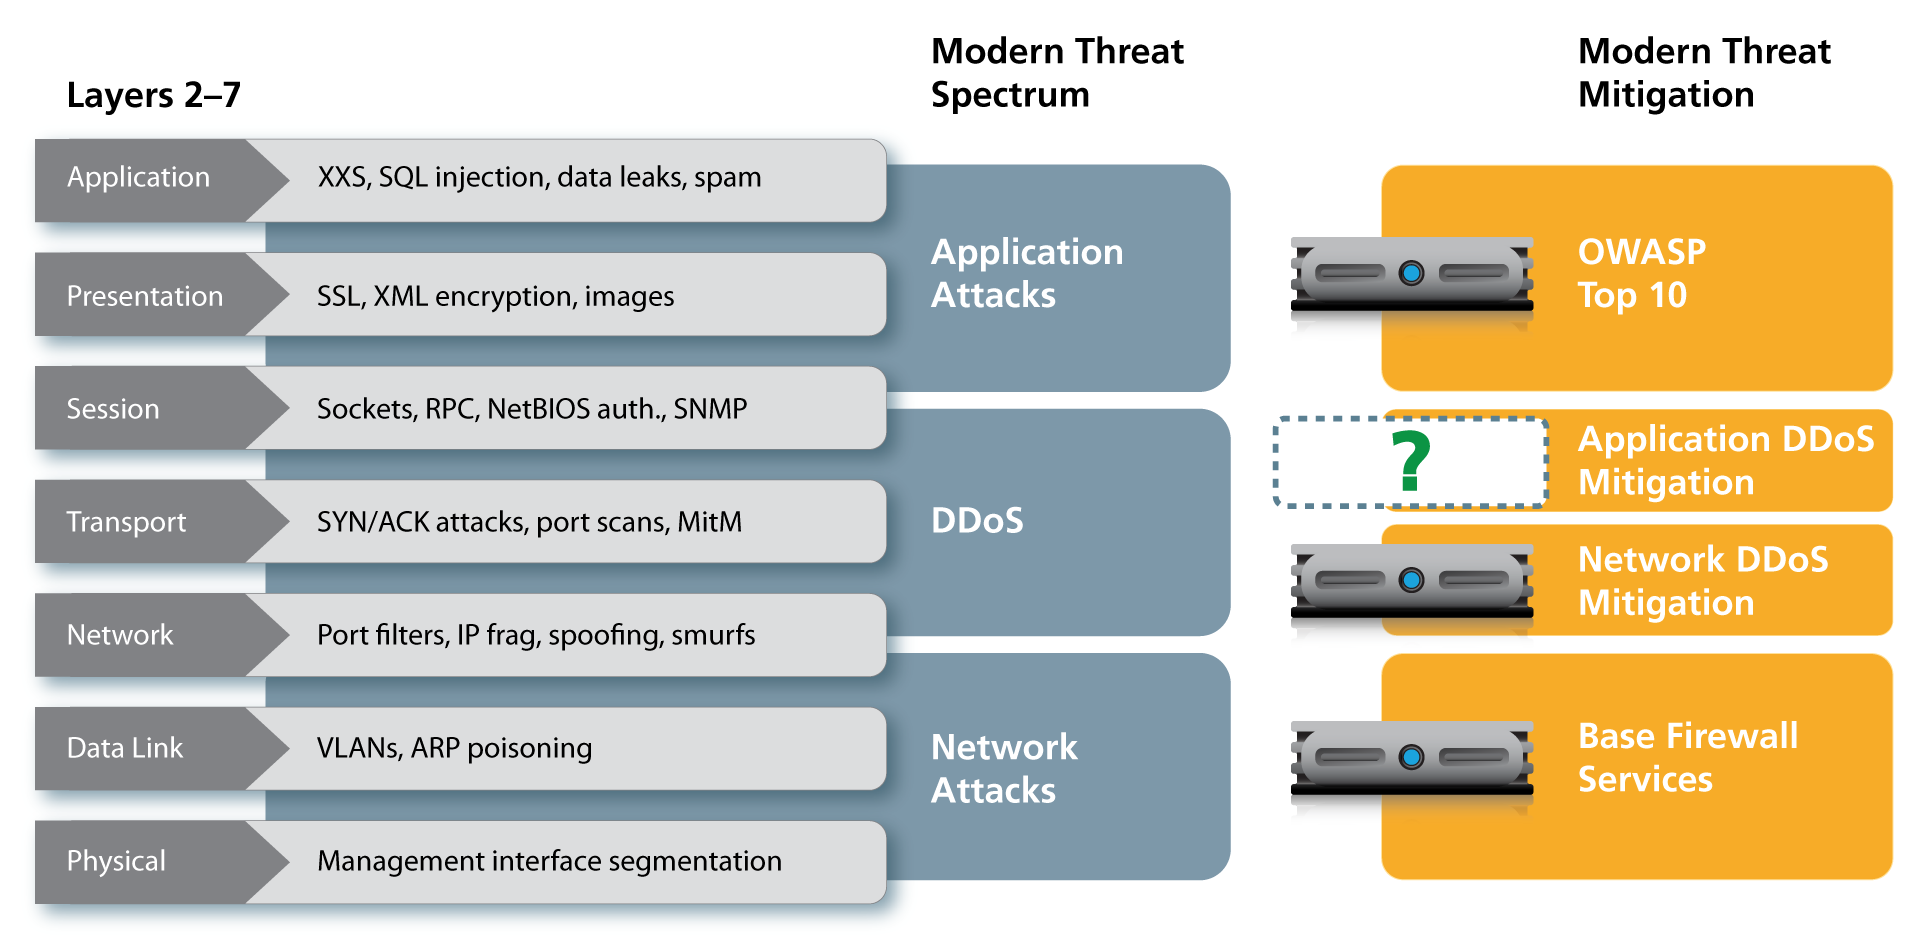
\includegraphics[width=450px]{./assets/img/osithreats.png}
	\caption{Possible threats at each OSI model layer and possible mitigation techniques.}
\end{figure}

Web threats can target any level of the OSI model in order to exploit different weaknesses or perform different types of attacks for various reasons (Figure \ref{fig:osithreats}).  Application attacks, which this research is focusing on, occur on the Application, Presentation, and partially the Session layers.  While several of these attacks can be mitigated by preventing the OWASP Top10 security flaws, it is only mitigation and there is always the possibility for a new attack variant to slip past.

Attacks will always prefer the most vulnerable target, the weakest link, and there is nothing more vulnerable than the public-facing application.  Studies have found that many of the existing techniques for handling these application layer attacks suffer from one or more of the following techniques:

\begin{itemize}
	\item Inherent limitations
	\item Incomplete implementations
	\item Complex frameworks
	\item Runtime overheads
	\item Intensive manual work requirements
	\item False positives and false negatives
\end{itemize}
% a survey on web application vulnerabilities
This means that despite the fact that these attacks are considered easy to mitigate, the existing solutions are not completely adequate for defending against some of the most common web attacks.  In order to solve this problem new methods of detection and prevention need to explored and older conventional methods need to be improved.

\section{SQL Injection}
Structured Query Language or SQL or short is the most dominant language for interacting with relational databases in recent years.  A SQL injection is an attack where through various means arbitrary unauthorized SQL code is ran on the database.  When one of the primary reasons behind performing these attacks is to gather confidential data this is an obvious means of acquiring the information.% a survey on web...
There are four common methods of injecting the SQL commands into the application:

\begin{itemize}
	\item Injection through user input
	\item Injection through cookies
	\item Injection through server variables
	\item Second-order injections
\end{itemize}

Injection through user input is the simpliest method, where the malicious user simply enters the arbitrary SQL code into any field that has some interaction with the database.  Injection through cookies involves applications that read from the cookie's fields to restore the users state, this information can be modified to contain SQL code to be read on returning to the website.  Injection through server variables such as PHP session variables, or other environment variables are used in a similar manner to cookies by applications and can be exploited in a similar fashion.  Lastly, second-order injections are some of the hardest to detect because they involve an attack that occurs later on after the data is entered. % A classification of SQL injection attacks

The impact and purpose of SQL injections can be broken down into four main categories.  First, \textbf{confidentiality} is lost, database that hold sensitive information which may be financial or identifiable is compromised and can now be considered public knowledge.  Secondly, in addition to the data being potentially leaked it now also has its \textbf{integrity} compromised as the malicious user can make any modification he wants to the data.  \textbf{Authentication} and \textbf{authorization} of the application is also broken, it is now possible to log in as any user with any access level, removing the need for passwords and bypassing any safe guards.

While SQL injections are commonly used to retrieve the information from a database, there are much more nefarious things that can be done with it.  For example, previous wide-scale botnet attacks have used SQL injections mimicing as Google queries to facilitate malicious drive-by-download attacks on websites to spread malware.  % a survey on web... 

\subsection{SQL Injection Types}

Often times many of these injection types are combined together and are not absolute, but the techniques can be classified under the six following categories.

\textbf{Tautology} attacks are designed to typically bypass authentication, identify injectable parameters or extract data.  It is typically done by using conditional SQL statements to evaluate to true in the WHERE portion of the query.  This will result in the query evaluating to true for every single row in the table and will often return all of them depending on how the application and the injection query is designed. For example the 1=1 portion of the following query will always evaluate to true:

\code{SELECT accounts FROM users WHERE login=’’ or 1=1 -- AND pass=’’ AND pin=}

A \textbf{malformed} or invalid query are often performed to gather information about the underlying database or applications structure to design more targetted queries.  This is due to the common mistake of having overly descriptive errors that reveal information that is very useful to an attacker. This can reveal information ranging from the DBMS used to the names of columns or tables.  The following example forces a conversion error:

\code{SELECT accounts FROM users WHERE login=’’ AND pass=’’ AND pin= convert (int,(select top 1 name from sysobjects where xtype=’u’))}

A third type of SQL injection exploits the \textbf{union} keyword which is used to combine rows of multiple tables.  This would often be used for extracting data as you can combine the data of another table which you only know a limited amount of information but is what you are interested in, with another table that is easily exploitable.  The following example combines the credit card information from another table with a null table, returning only the credit information which we are interested in:

\code{SELECT accounts FROM users WHERE login=’’ UNION SELECT cardNo from CreditCards where acctNo=10032 -- AND pass=’’ AND pin=}

\textbf{Piggy-backed} queries are where additional queries are added onto an existing query, this is the technique many people who have heard about when learning about SQL injections because it involves ending the current query and starting another.  This is typically done in the following syntax:
\code{; < Piggy-Backed Query > --} The semi-colon signifies the end of the current query, a new query is added, and then the remainder of the query is commented out, here is an example:

\code{SELECT accounts FROM users WHERE login=’doe’ AND pass=’’; drop table users -- ’ AND pin=123}

\textbf{Stored procedures} are typically designed to do something much greater than just extract data and instead do something much worse such as escalating themselves in the database environment or denying service.  Often times developers think that using embedded procedures makes their code protected from injections as all of the queries are within the database environment, but this is not the case. Given the following stored procedure to check our login credentials, we can inject \code{’ ; SHUTDOWN; --} and generate the following piggy-backed query.

\code{CREATE PROCEDURE DBO.isAuthenticated @userName varchar2, @pass varchar2, @pin int\\
AS\\
	EXEC("SELECT accounts FROM users\\
	WHERE login=’" +@userName+ "’ and pass=’" +@password+ "’ and pin=" +@pin);\\
GO}

\code{SELECT accounts FROM users WHERE login=’doe’ AND pass=’ ’; SHUTDOWN; -- AND pin=}

The last category are \textbf{inference} attacks, these are used where malformed queries cannot be used to provide vital information to construct attacks.  Instead, injections are preformed and the website is monitored for changes or a response, this information is used to deduce vulnerable parameters and information on the values in the database.  There are two types of inference attacks, \emph{blind injections} and \emph{timing attacks}. Blind injections are posing simple true or false queries to the database, if the query evaluates to true then nothing will change, but a false evaluation will typically differ in some way.  For example, the two following queries should both return an error if the input is handled properly, but if only the first one returns an error than the login parameter is vulnerable:  

\code{SELECT accounts FROM users WHERE login=’legalUser’ and 1=0 -- ’ AND pass=’’ AND pin=0\\
SELECT accounts FROM users WHERE login=’legalUser’ and 1=1 -- ’ AND pass=’’ AND pin=0}

Timing attacks make use of the \code{WAITFOR} keyword to note the increase or decrease in the response time instead of an error message.  The following example is trying to extract table names by using a binary search method, if there is a delay in the response then the attacker knows how to adjust his search.

\code{SELECT accounts FROM users WHERE login=’legalUser’ and ASCII(SUBSTRING((select top 1 name from sysobjects),1,1)) > X WAITFOR 5 -- ’ AND pass=’’ AND pin=0}

It is also important to note that any of these attacks and the future discussed attacks can also obscure their presence by using alternative encodings for the text that is entered, for example input can be converted to unicode or hexadecimal.
% A classification of SQL-injection attacks

\section{Cross-Site Scripting}

Cross-site scripting attacks or XSS for short are similar to SQL injections in that the arbitrary code is injected from user inputs but instead of influencing the database it will leverage the facing code of the web application, more often the HTML or Javascript.  XSS attacks can be used for a variety of purposes, to redirecting users to other websites or just simply changing the look of the website.  In the worst case, XSS attacks can be used to hijack users sessions to collect information from the user.

It is hard to pinpoint the level of impact of a XSS attack because it all depends on what it is being used for.  XSS attacks, unlike SQL injections can be just a minor nuisence or can be just as severe and collect sensitive information.  Often times instead of a XSS attack being used alone, it is instead used as part of a larger scheme to send a user to another attack website where a phishing attack or something of similar nature lies.
% a survey on web...
%xssdm...

\subsection{Types of Cross-Site Scripting Attacks}

The first type of XSS attack is called a \textbf{stored} or \textbf{persistent} attack.  These are attacks that are permanently stored in a database, whenever a user access the page that retrieves the information from the database they're browser runs the attack. A simple example is just inserting typical HTML code into a comment field.

The second type of XSS attack is referred to as a \textbf{reflected} attack.  Instead of the result being stored in the remote-server they instead originate from another source, sometimes an email link or another website, upon clicking the link the code runs as the browser considers it from a safe source.  These attacks are non persistent because you would have to click the original link again for the attack to run as it is not tied to the page like in a stored attack.
%OWASP XSS

The final type of XSS attack is a newer distinction for XSS attacks called a \textbf{Document Object Model (DOM) based} attack.  In this variant, the attack is ran through modifying the actual document model through javascript's document object.  What seperates this attack from a stored or reflected attack is the original page does not change, but instead of users actions will result in a different result because their environment has been modified.
%owasp DOM XSS

\section{Remote File Inclusion}

The final web-threat that will be examined in this research is remote file inclusion also known as RFI.  Put simply, it is using the vulnerabilities of the application to include remote files which may include arbitrary code of any language.  The most common example is abusing PHP's include() command to get some PHP code to run on the remote server.  RFI attacks allow for code execution on the remote server and client-side, denial of service attacks due to remote shells and data extraction.
% OWASP RFI

Whle there are not any predefined variants for RFI attacks, for the purposes of this research RFI attacks will be divided into the following three categories:

\begin{itemize}
	\item Only parameters with URLs
	\item Only paramters with PHP commands
	\item Parameters with URLs and PHP commands
\end{itemize}
 % drafted % web threats
\chapter{Current Detection and Prevention Methods} \label{sec:sectionThree}

\section{Prevention through Development} \label{sec:preventDevel}

Web attacks can be significantly damaging to an organization in many ways and so detection and prevention is of very high importance.  These attacks and subsequent problems are not only limited to only small time organizations as well, with many high profile websites are becoming victims to large but similar attacks as well.  Some studies state that over 90\% of web applications are vulnerable to SQL injections alone. \cite{detectionAndPreventionSQL}

The best way to stop these web attacks is to prevent the vulnerabilities from existing in the first place, this is accomplished on the development side.  Despite the fact that the majority of the attacks are well documented and understood, as safeguards are preventions are put in place to protect one aspect of an application, attackers shift their efforts to look for the next weakest area.  From a security standpoint you need to assume that your application is not bulletproof and that you have only mitigated the risk but never removed it completely.  As a result of this rationale, prevention alone is not enough as there is always the possibility that an attack finds a way past the safeguards and so detection must work hand in hand with prevention.

The simpliest and most common method to prevent these attacks targeting the application layer of the web application is to never allow user input to be directly concatenated into any command that interacts with the server-side.  This is done by making use of what is called prepared statements, you instead construct the entire query or command and then pass in your data from the user as parameters.  This allows the server to distinguish between data and code no matter what kind of input is supplied by the user.  Likewise, whenever data is accessed from storage to be displayed to the user, it should not be directly inserted into a command that could potentially treat it as arbitrary code.  This will prevent issues such as stored XSS attacks or RFIs from occuring where stored code is inserted into the flow of the application code.  \cite{owaspSQLPrevention}  Many languages have different ways of accomplishing this but the most simpliest way is to simply strip the portions that cause it to be interpreted as code, but a more comprehensive way is to filter the HTML against some form of filter or whitelist. \cite{htmlPurifier}

These are other measures that can be taken to mitigate the attacks but they mostly pertain to the environment on which the application is ran on and specifically for SQL injection prevention rather than all attack types.  Seperate database users should be made for each application and they should have the least amount of privledge possible.  In the event that something is compromised, that database is at least isolated and other applications are uneffected.  A second measure that can be taken is to use views extensively instead of using direct queries for all database interactions as it allows access to the tables to be denied and instead only to the specially tailored views.  These strategies embrace the least privledge concept, where it is an unnessecary risk to be privy to more information or have more access than you truly need. \cite{owaspSQLPrevention}

Research has been done on examining the code of potentially XSS vulnerable applications to determine their vulnerability and was able to accurately detect the vulnerable code with no false positives or negatives.  So it is clear that modifying the code itself to be more secure should always be the top priority if it is possible to determine if a particular file is vulnerable that easily and accurately. \cite{xssdm}

\section{Signature Based Detection} \label{sec:sigDetection}

A traditional and common way of detecting security threats is the use of signatures, however many of these signature based tools are more suited for the lower layers of the OSI model rather than the higher layers such as the application and presentation layers.  These tools are referred to as Intrusion Detection Systems (IDS) and many rely on regular expressions and other pattern matching techniques with signatures produced using previous attacks methods, one example of such a tool is Snort. \cite{mainPaper}  Therefore, as long as there is an adequate number of signatures that cover the broad spectrum of possible attacks then the detection approach can be quite successful.  

However signature based detection systems as well as other IDS systems are not completely fail proof.  One of the biggest problems is the frequency of false positives, or in other words when the system believes that something that is not harmful is harmful.  Of course the opposite is also true and IDS systems can let attacks slip by unnoticed, this can be a result of the attacks using various tricks to evade detection such as using alternate encodings or fragmenting packets or just simply being a new form of attack. \cite{onTheVerification}  In addition, if the IDS is signature based than what is a more likely explanation for these accuracy problems is a lack of signatures that are either more accurate or cover these new undocumented attacks.  It is becoming too impractical to produce these signatures fast enough due to the countless variants of the attacks and they are commonly designed to go unnoticed rather than spread as fast as possible like with conventional malware. \cite{trendMicro}  To give an idea on how difficult of a problem this is to solve with signatures alone, an average of 5,000 new software vulnerabilities have been identified per year; along with the number of unique malware programs alledgely in the tens of millions and doubling every year.  With these rapidly rising trends, it is clear that the malicious user is easily always ahead of the detection tools.  Static solutions including signature sets are becoming less and less practical every year for these reasons, and the current short comings of the detection systems to keep up themselves proves that point further. \cite{onTheVerification}

However, this problem is not unique to the web threat world, although signature based detection is much more suited for the traditional desktop computer application virus scanning practices have had to adapt as well to a similar problem.  Virus scanning is probably the best example of signature based detection in action, where malware is collected, a signature is developed to detect it, and then sent out to the masses as fast as possible.  However, some types of viruses have begun to exploit this by transforming their own code when transferring which would require an entire new signature to detect.  These so called metamorphic viruses are not impossible to defeat but they require approaching the idea of scanning for a virus completely differently than just collecting a single signature.  Such techniques include but are not limited to hidden Markov models or reversing the morphing process of the malware itself. \cite{metaInvincible} \cite{metaHunting}  If the area where signature based detection has proven to be the most strongest has had to adapt it's tactics to deal with the changing security climate, then by extension so to it does the web threat detection ecosystem.

\section{Modern Methods of Detection}

In order to overcome these challenges for detecting web threats, some people have suggested that a multiple layered approach will provide the best defense.  Such a system would not only have multiple layers of detection involving signatures and other techniques but also feedback loops to update the protection systems for improved future detection.  A multi-layered approach would also be able to address all levels of the network rather than a single system that can only handle a subset of the layers such as the network or application layers.  This approach would also enable portions of the processing to be centralized and in the cloud while other areas are closer to the endpoints.  Traditional techniques like signature detection would still be used, but it would be able to be augmented with additional techniques such as behaviour analysis as often times web attacks are carried out in massive enumeration attempts and not just a single bad request.  One final point is that such a solution would allow for global collaboration to contribute to reputation lists, whitelists, and the like to further solve the problem of a growing threat instead of having the same tools deployed in multiple areas and poor solutions for consistent updates. \cite{trendMicro}

A multi-layered approach combines the best of the old traditional techniques with new potentially better solutions, and even more interestingly suggests a system that can inherently learn and improve as a core trait; very similar to the technique in question in this research.








 % drafted % detection methods
\chapter{Describing Machine Learning Approaches} \label{sec:sectionFour}

\section{Machine Learning} \label{sec:machineLearning}

Machine learning has become a popular topic in recent years as an answer to the sheer amount of data that has the potential to be processed.  Not only does the large amount of data require more advanced and intelligent ways to process it, but there is also a big incentives driving the desire to do so.  Through machine learning techniques and patterns additional meaning can be extracted from the data which can be used to draw conclusions or predictions. \cite{dataManagementSystems}  Machine learning techniques are commonly applied to data mining tasks, examining at data and discerning additional information from it.  In the case of this research's problem area the data being mined is the large amount of web requests.

This brings numerous benefits to a security application such as web threat detection, primarily it allows the system to have some sort of feedback mechanicism to improve its detection and perhaps even it's prevention.  A system that is unable to learn overtime will not be able to overcome new techniques designed by attackers to evade the current detection systems abilities unless it is manually updated.  And as discussed before, manual updating is not only a very inefficient time consuming task but it is also just plain infeasible as the number and complexity of these attacks grows.  Identifying patterns from data is very useful when it's consider that many attacks follow some kind of a basic syntax or format and while there are many ways to evade detection, typically there is still a common method or intent that can be identified.

The way machine learning operates is by identifying a series of features in the data set in question, these features are then used by the algorithm learn and make better decisions.  The key distinction of machine learning is that the algorithms are not told what to do explicitly but instead is allowed to make its decision based on measurements such as performance. \cite{supervisedMachineLearning}
  
\subsection{Supervised Learning} \label{sec:supervisedLearning}

Machine learning algorithms can either make use of supervised learning or unsupervised learning.  In supervised learning the system is provided with labelled data, data that states what the end result should be so that the system can be accurately trained without additional intervention.  There is also another type of learning called reinforcement learning where an external source informs the system how well it is working or not as it progresses.

Supervised learning has issues that must to be overcome however, the first of which being collecting the original data set.  If there is prior research or people in the know that can suggest what features to use, then the process is much more trivial, otherwise the features are often identified using a brute force method.  The problem with using a brute force method other than the computation time is that the data has the potential to be noisy and miss important features which can lead to further problems.  Learning from extremely large datasets is very inefficient as well.  Therefore it is often desired to minimize the  size of the data set while still maintaining the final performance of the system through a process is called instance selection.  Lastly, having a large amount of features in the data set can also increase the complexity of the system.  To solve this irrelevant and redundant features should be removed whenever possible, but if many of the features depend on each other then they shouldn't be removed as this can lead to inaccuracies in of the learning process.  To deal with features that can't be removed,, new features can be constructed or existing ones altered to be more concise and accurate, improving the entire system as a whole.

One of the big steps in creating a machine learning system is selecting the right algorithm for the dataset, each which their own advantages, disadvantages and times where they are applicable (Section \ref{sec:sectionSeven}). 

\section{Genetic Algorithm} \label{sec:genAlgorithm}

A genetic algorithm is a search-based algorithm that makes use of machine learning in order to locate optimal or near-optimal solutions for a particular problem.  This is what is meant by the term 'search' that is often used to describe this and other algorithms such as local search or simulated annealing, it is not about locating something in a particular data set but rather searching for the best possible answer.  Such algorithms, especially in the case of a genetic algorithm use fitness functions and possibly reward systems to distinguish between a better solution and one that should not be considered going forward. \cite{searchBasedSoftwareEngineering}

As the name suggests, a genetic algorithm mimics how genetic development in the real world works and how species evolve over time.  The algorithm begins with an initial population of individuals, an individual being a possible solution to the problem in question.  Every individual has it's fitness evaluated using some form of calculation tailored to suit the problem at hand; for our purposes for web threat detection the fitness will be evaluated with the following:

\begin{algorithm}[H]
	\setstretch{1.0}
	\centering

	$fitness = (\frac{correct\ detections}{\alpha})\ - (\frac{false\ positives}{\gamma})\ - (\frac{incorrect\ detections}{\beta \cdot 8})$ \\
	
	$\alpha \leftarrow The\ number\ of\ possible\ correct\ detections$ \\
	$\beta \leftarrow The\ number\ of\ possible\ incorrect\ detections$ \\
	$\gamma \leftarrow The\ number\ of\ possible\ false\ positives$ \\
	
	\caption{Fitness algorithm for use in genetic algorithm}
	\label{alg:fitness}
	\vspace{2cm}
\end{algorithm}

Correct detections with improve the fitness of a particular individual and the individual is more likely to be selected for genetic operators later on, where as false positives and incorrect detections impact the fitness negatively, with incorrect detections having less of a negative impact than the former.  As an example, if we are looking for SQL injections, every deleted request that is a SQL injection is correct, if instead it isn't an attack at all then it is a false positive and if it is actually a XSS or RFI attack then this is an incorrect detection.

In order for the genetic algorithm to produce a new population it makes use of what are called genetic operators which commonly include performing crossovers and mutations to the individuals.  Two individuals at a time in the population are selected by a selection algorithm and crossed over, there are many ways to perform a crossover but a single-point crossover will be the method used for this research.  A position is selected to perform the crossover, referred to as a locus, for our purposes this refers to selecting a segment, this segment is then swapped with the other selected individual's respective segment to produce two new individuals with unique chromosomes, or in other words different configurations.  This process continues until the algorithm has produced enough new individuals to fill the next population, in addition, at the beginning of this process it is possible to mark some of the top individuals as elite and bring them into the new population unaltered.  Before continuing to the next generation every single allele, or piece of information in each individual has a small chance to be mutated, this is what causes the population to have some sort of diversity.  This entire process then repeats many times, each time being referred to as a generation and by the end of the process there should be a set of individuals that are closer to solving the problem.\cite{matlabGenetic}

\subsection{Current Genetic Algorithm Solutions} \label{sec:currentGenSolutions}

These genetic algorithm techniques have been applied to web threat detection already, one particular paper focused on using variants of an attack to detect network related attacks.  While they may not have directly used a genetic algorithm in their solution, the core idea is very similar to how a genetic algorithm operates with generating different individuals and seeing if they fit a certain criteria.  These exploit variants were used to test signature based detection methods to see if it was possible to evade them and results showed that it was.  This is proof that traditional models for detection cannot be made absolutely perfect and that the using an approach similar to genetic algorithm technniques is worthwhile for atleast evading detection. \cite{testingNetworkBased}

As of recently research has taken this idea and done the opposite, using a genetic algorithm directly to detect web attacks rather than to evade detection.  The genetic algorithm was used to make variants of attack detection signatures that can best detect SQL injections, XSS, and RFI attacks through the text-based web request logs.  The results of which were very promising with around a 90\% detection accuracy reported which exceeded the performance of a traditional regular expression signature based detection system. \cite{mainPaper}

These recent findings are the starting point for this research, improving the genetic algorithm approach and gathering more detailed results about it's function and performance, as well as being the comparison point for another machine learning technique, support vector machines.

\section{Support Vector Machine} \label{sec:SVM}

A support vector machine's main technique for classifying data is to divide the data set into two or more categories with the largest margin possible between the seperation(s), referred to as a hyperplane(s).  The reason for maximizing this buffer between categories is to reduce the chances of classification error as much as possible.  With the hyperplane(s) computed, points that lie within the margin are referred to as support vectors, hence the name, and it is these points which were used to calculate the hyperplane(s) in the first place with the other data points being ignored (Figure \ref{fig:svmmargin}).  

\begin{figure}
	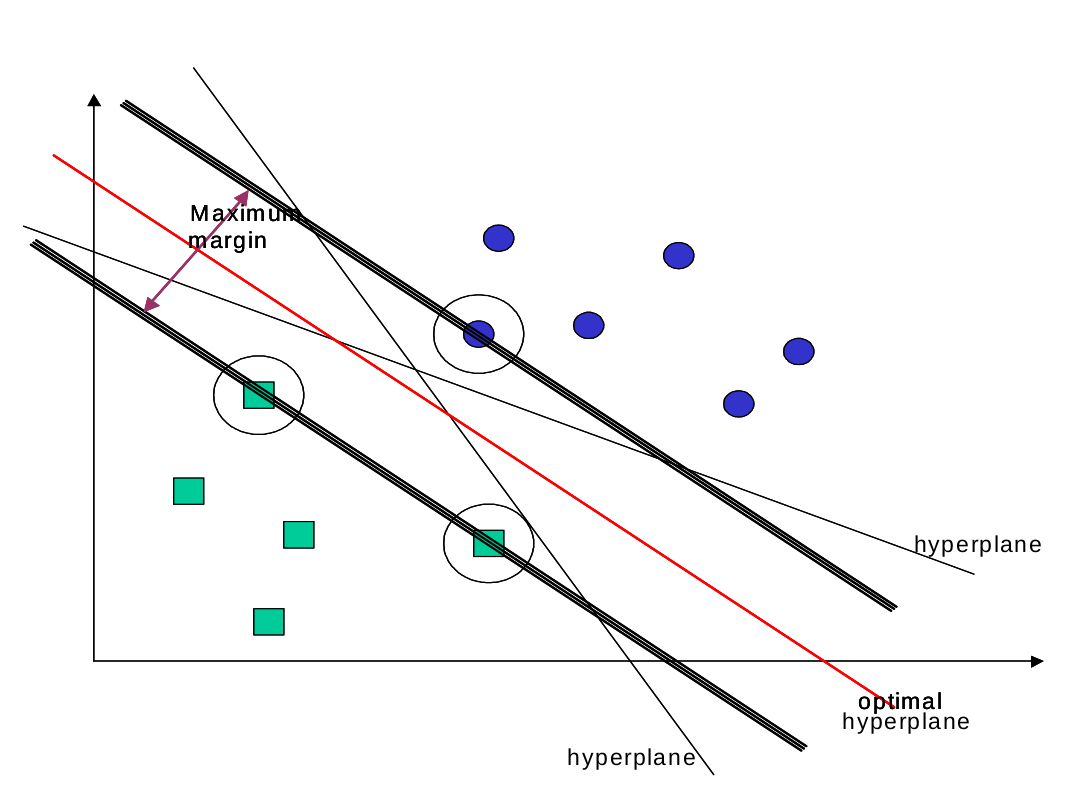
\includegraphics[width=450px]{./assets/img/svmmargin.png}
	\caption{Example of a linear seperated SVM}
	\label{fig:svmmargin}
\end{figure}

The fact that the SVM is determined by only the support vectors which are usually a very small subset of the training vectors, is great because it means that the speed does not significantly slow down with a larger amount of features.  However it is also realistic to imagine data that cannot be easily divided, this can be solved using soft margins that allow for misclassifications or in more complex cases the data can be mapped to a higher dimensional space to open up other options of dividing the data.  This higher dimensional space is referred to as the transformed feature space, however simple linear seperations in the higher dimensional space transform into non-linear seperations when you return back to the original space.  

If this feature space data is mapped to a Hilbert space referred to with $\Phi$, which allows for traditional euclidean space vector calculations to be extended to an infinite amount of dimensions using dot products using equations in the form of: $\Phi\left(x_i \right)\cdot\Phi\left(x_j \right)$.  This means that we can use what is called a kernel function to avoid ever having to determine the mapping to $\Phi$ and calculate the necessary results directly in the feature space instead.  A kernel function is in the form of: $K(x_{i},x_{j}) = \Phi(x_i) \cdot \Phi(x_j)$. \cite{supervisedMachineLearning}  There are many commonly used kernels, three of which will be used in this research: linear, polynomial (with degree 3), and radial basis function (Table \ref{tab:kernels}).  

\begin{table}[h]
	\centering
	\begin{tabular}{|p{1.5in}|p{4.5in}|}
	\hline
		\textbf{Kernel Function} & \textbf{Mathematical Formula}\\
	\hhline{|=|=|}
		Linear  & $K(x_{i},x_{j}) = \langle x_{i},x_{j}\rangle$ \\
	\hline
		Polynomial & $K(x_{i},x_{j}) = (\langle x_{i},x_{j}\rangle + 1)^d, d: degree$ \\
	\hline
		Radial Basis Function (RBF) & $K(x_{i},x_{j}) = \exp\left(\frac{- \parallel x_i - x_j \parallel^2}{2\sigma^2} /\right), \sigma : width\ of\ RBF\ function$ \\
	\hline
	\end{tabular}
	\caption{Kernels that will be used and their mathematical function} \cite{intrusionDetectionCostBased}
	\label{tab:kernels}
\end{table}

Once the SVM is trained using a kernel method of choice the only step left is to pass in all of the testing data and see which side of the hyperplane(s) it falls in order to classify it.  An SVM can at times get very computational intensive and can run very slow, this is often due to the choice of the kernel function as well as the parameters that influence the kernel.  For example, a linear kernel is very simple where as an RBF kernel is much more complex.  Two parameters that are worth mentioning for the SVM training process are $\gamma$ (gamma) and C.

Gamma is used in the polynomial and RBF kernels to define how much influence each training vector has on the seperating hyperplane(s).  A lower gamma value corresponds to a far influence, when gamma is too small the influence of any support vector may extend to the entire set and the end result would instead just be regions of high density being isolated from other high density areas.  On the converse if gamma is too high then the influence would only extend to the support vector itself.  The C parameter is the penalty cost assocated with misclassification, if C is low then classification is more relaxed compared to a higher C which will encourage more support vectors to be chosen and achieve a more accurate division. \cite{rbfSVMParameters}  There is no way to know what are the best values to choose for gamma and C because it depends on the dataset in question and so this must be done by doing testing.

\subsection{Current Support Vector Machine Solutions} \label{sec:SVMSolutions}

Support vector machines have also been applied to web threat detection as well but only in the lower layers of the OSI model dealing with network related attacks such as denial of service.  One such study used a cost based support vector machine to detect web attacks and was able to detect them with an overall accuracy of 99\%. \cite{intrusionDetectionCostBased}  Likewise, another study compared the usage of an SVM versus an artificial neural network and found that the SVM was much faster in comparison along with achieving a 99\% accuracy as well. \cite{intrusionDetectionNeural}  These results of these two studies show that the SVM approach is a viable one and can be used for practical applications with detection web threats, so it will be interesting to see how well the algorithm performs for application layer attacks as well as how it compares to the genetic algorithm approach.


 % drafted % machine learning
\chapter{Methods \& Procedures}

\section{System Overview}

Despite the fact that two rather different algorithms will be used the system is designed to operate more or less the same with the genetic algorithm or support vector machine components as loosely coupled modules to avoid having to redesign the system for both approaches.  Web requests will be processed through a parser that looks for various aspects related to each of the three possible web attacks.  The results are then output and can be used as input for either the genetic algorithm, support vector machine, or potentially another algorithm that could extend the testing.  Finally, the testing modules will output the results to a file that can be processed by graphing tools (Figure \ref{fig:sys}), in this case the R programming language will be used to create graphs that can be used to drawn conclusions on the two approaches. % cite R

\begin{figure}
	\label{fig:sys}
	\includegraphics[width=450px]{./assets/img/system.png}
	\caption{Overview of the system}
\end{figure}

\section{Gathering Test Data}

All data will be gathered from as close to a real-world scenario as possible.  In order to do so, automated enumeration exploiting tools will be used to gather a large sample size of varied attacks (Table \ref{tab:tools}).  
In order to gather SQL injection attacks the popular tool sqlmap will be used, for XSS attacks Grabber and XSSer will be used. %cite the tools
These tools will be let loose on a private apache web-server that is hosting a very simple database connected application. %cite apache
In regards to gathering a large amount of RFI attacks it will require generation of a large sample size, as the tooling for these types of attacks is rather limited and the tools that do exist do not perform large scale enumeration attacks and instead attempt to compromise the server as fast as possible. % cite fimap
Because RFI maps are the simpliest in terms of their design and variations, a simple automated Python script can be used to generate a large amount of attacks using a heavy amount of randomization.  Finally, it is nessecary to also include some normal web requests which are not attacks to test for false positives.  This can easily be done by using the application as well as other websites normally, submit form inputs, etc, and collecting all of the resulting HTTP requests.  This can be done with a browser extension for Mozilla Firefox, HTTPFox. % cite http fox

\begin{table}
	\centering
	\label{tab:tools}
	\begin{tabular}{|l|l|}
	\hline
		\textbf{Request Type} & \textbf{Generation Method}\\
	\hhline{|=|=|}
		SQL Injection & sqlmap\\
	\hline
		XSS Attack & grabber, xsser\\
	\hline
		RFI Attack & randomized generation\\
	\hline
		Normal Requests & httpfox\\
	\hline
	\end{tabular}
	\caption{Breakdown of test data generation}
\end{table}

Like most web-servers, Apache has the ability to log all of the requests that it serves to a file.  The data that we need to parse for the genetic algorithm or support vector machine is the GET or POST HTTP request line.  The final step of gathering the testing and training data is to compile the log files and strip out the unneeded information so it can be passed to the parser.  Another small Python script can be used to generate a test file using these large banks of the correct size and proportions, this script will generate a file where each line contains the request line content and what type the request is, either SQLi, XSS, RFI, or not an attack.

\section{Parsing the Requests}

With the completed test file(s) containing the proper amount of each attack and normal requests, the next step is to parse each request into numeric values so that the algorithms can work on them.  Each request has their own respective features that are worth identifying, with more features needing to be identified for the genetic algorithm than for the SVM.  These features have been identified for each request type by previous research (Table \ref{tab:features}) but is important to distinguish the meaning of each as well as what can and cannot be detected in this way. % cite main papaer

\begin{table}
	\centering
	\label{tab:features}
	\begin{tabular}{|p{1.5in}|p{4.5in}|}
	\hline
		\textbf{Request Type} & \textbf{Features}\\
	\hhline{|=|=|}
		SQL Injection & \# SQL keywords, is encoded, \# fields containing SQL keyword, attack variant\\
	\hline
		XSS Attack & \# of HTML or javascript keywords, is encoded, \# fields containing a HTML or javascript keyword, attack variant\\
	\hline
		RFI Attack & \# of URLs, is encoded, \# of commands, attack variant\\
	\hline
	\end{tabular}
	\caption{Parseable Features}
\end{table}

The number of SQL keywords or reserved words is obtained by using a comprehensive list provided by the Oracle and MySQL DBMS documentation. % cite Oracle and MySQL documentation
This works well with our test environment as well, as the DBMS our application is using is MySQL so many of the automated attacks will use MySQL specific vulnerabilities.  Similarly, the HTML and javascript keywords were provided by the official W3C documentation and the official PHP related commands were sourced from PHP's main documentation.  % cite W3schools and php docs

Requests are capable of being encoded as well to further evade detection (Section %site chapter).
and so this is something that can be easily detected and recorded.  HTTP requests, usually GET requests specifically, will contain along with them fields and the information that they carry to the application code.  This information can be user supplied information (ex. a username or password) or application supplied information (ex. the current page number), either way it is able to be directly modified by a user and is where injections and malicious code is likely to lie (Figure \ref{fig:sampleRequest}).  For this reason, it is good to make a distinction between just a total number of keywords found and the number of fields that actually contain keywords to get a more complete picture.  Lastly, all of the discussed attack variants (Section % cite the chapters with it).
can be detected with the exception of \emph{Stored Procedure SQL injections}, which brings up the limitations of this type of parsing (Section % cite chap 7. 

\begin{figure}
	\centering
	\label{fig:sampleRequest}
	https://duckduckgo.com/?\hl{q=HTTP+Request}\&\hl{t=vivaldi}\&\hl{ia=web}
	\caption{A sample HTTP request with fields highlighted}
\end{figure}

The parser makes heavy use of regular expressions (Appendix A % cite)
to determine much of this information such as the keywords or contents of the fields and is designed to overcome common evasion tactics.  One such tactic is padding the alternate encodings of the request, instead of using the common two byte hexadecimal conversion of the ASCII values, several zeros can be appended to the two bytes to confuse simple parsers using built-in decoding libraries.  Another issue that had to be overcame was not double-counting keywords that were a prefix to another keyword, which is done simply by associating each word with its prefix combinations.  This results in only a minor amount of extra computation as there is not many keywords with prefixes.

\begin{algorithm}[H]
	\setstretch{1.0}
	\label{alg:parsing}
	\caption{General overview of parsing procedure}
	
	\KwData{File with HTTP Requests and their true type}
	\KwResult{Resulting test file with every request stored along with the parsed features for the three types of web threats in the follwing order Original > SQLi > XSS> RFI}
	
	read in input file\;
	\For{line in input file}{
	
		\If{for SVM testing}{
			disregard encoding and attack variant features\;
		}
		pass request to each parsing module (sql, xss, and rfi)\;
		store original request and type in resulting file\;
		\For{each parsed result}{
			\eIf{for genetic algorithm}{
				
				\eIf{lengths of segment 1 and 3 should be permuted for length testing}{
					\For{each segment length combination up to specified maximum}{
						convert result to binary based on the maximum lengths of each segment\;
						\If{decimal value exceeds maximum value in segment}{
							use maximum allowed value in segment\;
						}
						store result in a list\;
					}
					store complete list on a new line\;
				}{
				convert result to binary based on the maximum lengths of each segment\;
					\If{decimal value exceeds maximum value in segment}{
						use maximum allowed value in segment\;
					}
				store complete bitstring in file on new line\;
				}
			}{
			store decimal values into file on new line\;
			}
		}
	}	
\end{algorithm}

Full documentation on the usage of the parser (Appendix). % forward reference

\section{Genetic Algorithm Based Signature Detection}\label{sec:genIntro}

The method of the using a genetic algorithm for signature based detection is largely the same as the proposed and tested system in previous research with a few modifications. %cite main paper
One major difference is that instead of allowing the signatures to change to different attack type signatures (ex. SQLi to XSS) we specify what type of attack we want to search for and the algorithm uses that parsed result for every request.  This of course requires every original request to be parsed three times instead of just once, but it makes the most sense as if it is possible to transition between attack types so easily then there is no reason to differentiate between them in the first place.  This also causes later conclusions to not be influenced by factors that can not be measured.  If signatures were allowed to switch to different attacks types then it would be unknown if the results were due to the random nature of a genetic algorithm or the other variables being changed.  

The second major change is that the bitstring length for each signature is increased to avoid problems of exceeding the quantity in a segment.  In the previous research only 3 bits were used for the segments that count the number of segments or fields in the requests which only allows for a count up to 7.  In a real world setting the amounts for the number of fields and keywords can be much much larger and exceeding these values often creates a situation where there are many signatures that match which normally would not.  For example, if two signatures have 10 and 11 keywords respectively, with the old segment lengths they would be capped at 7, or 111, resulting in a match which should not have occured.  Therefore these segment lengths with a size problem have been extended to 6 bits allowing for counts up to 63 (Table \ref{tab:geneticSegments}).

\begin{table}
	\label{tab:geneticSegments}
	\begin{tabular}{|p{1.5in}|p{1.125in}|p{1.125in}|p{1.125in}|p{1.125in}|}
	\hline
	\multicolumn{1}{|p{1.5in}|}{\textbf{Request Type}} & \multicolumn{4}{p{4.5in}|}{\textbf{Segment Information}} \\ \hhline{|=|=|=|=|=|}
	\multirow{2}{*}{\textbf{SQL Injection}}            & \# of SQL Keywords & is encoded & \# of fields containing a SQL keyword & attack variant \\ \cline{2-5} 
		                                      & 6             & 1          & 6            & 3 \\ \hline  
	\multirow{2}{*}{\textbf{XSS Attack}}               & \# of HTML or javascript keywords & is encoded & \# of fields containing a HTML or javascript keyword & attack variant \\ \cline{2-5} 
		                                      & 6             & 1          & 6            & 3 \\ \hline
	\multirow{2}{*}{\textbf{RFI Attack}}               & \# of URLs & is encoded & \# of PHP commands & attack variant \\ \cline{2-5} 
		                                      & 6             & 1          & 6            & 3 \\ \hline  
	\end{tabular}
	\caption{Genetic algorithm default segment breakdown}
\end{table}

The genetic algorithm implemented is very standard, allowing for the following parameters to be changed:

\begin{itemize}
	\setstretch{1.0}
	\item Maximum population per iteration
	\item Maximum number of generations
	\item Number of iterations
	\item Mutation rate
	\item Elitist selection amount
\end{itemize}

Most of the genetic operators are fairly simple to implement with the most complex being selection.  The higher the bitstrings fitness is the more likely it should be selected.  There are several ways for this to be accomplished but for this implementation Roulette Wheel Selection is used, also referred to as Fitness Proportionate Selection (Algorithm \ref{alg:selection}).  This selection algorithm was choosen as the originally proposed genetic algorithm technique was fitness based %cite main paper
 and not reward based like other selection algorithms, as well as it is simple to implement and understand for these basic testing purposes.  For crossovering two individuals a single point crossover scheme is used.

\begin{algorithm}[H]
	\setstretch{1.0}
	\label{alg:selection}
	\caption{Basic pseudocode algorithm for Roulette Wheel Selection in \BigO{n}}
	\KwData{Fitness values of all individuals in population}
	\KwResult{The selected individual}
	
	$totalWeight\leftarrow0$\;
	\For{all individuals weights}{
		$totalWeight\leftarrow$totalWeight + weight\;
	}
	
	generate a random number between 0 and the totalWeight\;
	\For{all individuals weights}{
		
		subtract the weight from the random number\;
		\If{random number is less than 0}{
			return that individual
		}
	}
	
	\If{Unable to find an individual, error occured}{
		fall back condition is to return the last item\;
	}
\end{algorithm}

The genetic algorithm was written from scratch using the Python programming language and is designed to handle input files with single bitstrings from the parser or lines with several variations on the lengths of the bitstrings (Algorithm \ref{alg:genetic}).

\begin{algorithm}[H]
	\setstretch{1.0}
	\label{alg:genetic}
	\caption{Pseudocode algorithm for genetic algorithm}
	\KwData{Bitstrings for training and testing and all parameters for genetic algorithm}
	\KwResult{The optimized bitstrings that can be used for detection}
	
	\For{each bitstring of varying length}{
	
		\For{the number of generations}{
			
			remove duplicate bitstrings in the current population\;
			evaluate fitness for all individuals\;
			
			preserve the top elitist percentage into the new population called the offspring\;
			
			\While{offspring amount is less than maxmimum population allowed}{
				
				locate two individuals and perform a single point crossover \;
				add these two new individuals to the next population
			}
			
			trim the offspring to the maximum population just incase\;
			
			loop through every bit in every offspring with the chance to mutate it\;
			
			set the current population to the offspring
		}
		
		store the bitstring results for that length
	}
\end{algorithm}

\subsection{Testing Procedure}

In order to the test the genetic algorithm fairly, both training data and testing data will have equal proportions of all three attacks, 30\% for each attack and then 10\% of non attacks for false positive metrics (Table \ref{tab:trainingfile} \& \ref{tab:testfile}).  In addition, the testing data will be different requests than that used in training as this is the situation that these approaches would be exposed in the real world.  They would be trained using supervised learning and then used to identify unlabeled data entering the system so it does not make sense to test with the same data it is trained on.

\begin{table}
	\centering
	\label{tab:trainingfile}
	\begin{tabular}{|p{1.5in}|p{1.5in}|}
	\hline
		\textbf{Request Type} & \textbf{Number in Sample}\\
	\hhline{|=|=|}
		SQL Injection & 300 \\
	\hline
		XSS Attack & 300 \\
	\hline
		RFI Attack & 300 \\
	\hline
		Non Attacks & 100 \\
	\hhline{|=|=|}
		\textbf{Total} & 1000 \\
	\hline
	\end{tabular}
	\caption{Breakdown of the training file for genetic algorithms}
\end{table}	
	
\begin{table}
	\centering
	\label{tab:testfile}
	\begin{tabular}{|p{1.5in}|p{1.5in}|}
	\hline
		\textbf{Request Type} & \textbf{Number in Sample}\\
	\hhline{|=|=|}
		SQL Injection & 1500 \\
	\hline
		XSS Attack & 1500 \\
	\hline
		RFI Attack & 1500 \\
	\hline
		Non Attacks & 500 \\
	\hhline{|=|=|}
		\textbf{Total} & 5000 \\
	\hline
	\end{tabular}
	\caption{Breakdown of the testing file for both genetic algorithm and support vector machine}
\end{table}	

Every test will make use of the same training data and testing data and instead the parameters for the genetic algorithm will be altered to see if they make a difference on the results.  The genetic algorithm will be trained using the training data, which will output bitstrings that act as signatures that are optimized for detecting the particular attacks. Those signatures will be used to hopefully match correctly with the unseen testing data (Figure \ref{fig:gasys}).

\begin{figure}
	\label{fig:gasys}
	\includegraphics[width=450px]{./assets/img/gasys.png}
	\caption{Overview of the genetic algorithm system}
\end{figure}

In addition to the various parameters to the genetic algorithm having multiple iterations of the algorithm ran to generate a combined amount of signatures will be tested.  The thought is that the more signatures in your detection set the more likely you are to have one to detect the attacks so more iterations combined together should be able to detect more attacks.  This is also one of the main reasons why this technique was proposed, so that the genetic algorithm could generate additional signatures automatically for testing instead of relying on manually made patterns.  Also, testing the results with different lengths of bitstrings will also be attempted, the thought here goes back to the problem of overflowing a segment (Section \ref{sec:genIntro}).  Small segments should be able to detect more attacks as they should be able to more easily generate bitstrings that cover a wider range of attacks.  For example, a segment that can only hold a count of 1 would detect anything if it contained a keyword even if that request had a much greater amount, it would essentially become a flag.

\section{Support Vector Machine Detection}

The SVM detection will follow a similar process to the genetic algorithm but instead of changing the parameters of the algorithm, the training data will be changed instead.  This is because the parameters for the SVM that will make a difference are automatically optimized by a grid search approach provided by the same library used to implement the SVM in Python. %cite scikitlearn

SVM use various different kernel methods to determine a pattern in the given data, the kernels that will are being used from the provided library is a linear, polynomial degree 3, and RBF kernels.  This will be the only parameter that will be changed for the SVM but every test is ran on each kernel so it is consistent throughout the entire process.  The parameters for the SVM that are optimized by the gridsearch are gamma and the penalty cost, gamma only effects the polynomial and RBF kernels however.

The one main difference between the SVM and genetic algorithm approaches is that the SVM only requires two of the four segments and it does not need to be in binary form to support mutations (Table \ref{tab:svmSegments}).  These values are plotted on a simple X,Y plane which is then passed into the SVM to be trained, each of these values is labelled data cooresponding to either it is an attack or it is not (Algorithm \ref{alg:svm}).

\begin{table}
	\label{tab:svmSegments}
	\begin{tabular}{|p{1.5in}|p{2.25in}|p{2.25in}|}
	\hline
	\multicolumn{1}{|c|}{\textbf{Request Type}} & \multicolumn{2}{p{4.5in}|}{\textbf{Segments}}               \\ \hhline{|=|=|=|}
	\textbf{SQL Injection}                      & \# of SQL Keywords         & \# of fields containing a SQL keyword \\ \hline
	\textbf{XSS Attack}                      & \# of HTML or javascript keywords         & \# of fields containing a HTML or javascript keyword \\ \hline
	\textbf{RFI Attack}                      & \# of URLs         & \# of PHP commands \\ \hline
	\end{tabular}
	\caption{Genetic algorithm default segment breakdown}
\end{table}

\begin{algorithm}[H]
	\setstretch{1.0}
	\label{alg:svm}
	\caption{Pseudocode algorithm for support vector machine}
	\KwData{Segment information for each request}
	\KwResult{A trained SVM classifier that test data can be passed into and results gathered with}
	
	gather all segment information from training set\;
	
	pack into a numpy array\;
	
	\For{each kernel type ('linear', 'polynomial-3', 'rbf')}{
		
		\If{that kernel type has not already had its parameters optimized}{
			optimize using a GridSearch\;
			store the resulting parameters to save time on the next repeat use of the kernel\;
		}
		
		build the svm using scikit-learn and the optimized parameters\;
		train the classifier using the training vectors and targets\;
		
		pass all testing data through the classifier and record results\;
		
		plot the resulting graph for visual purposes\;
		store results of testing\;
	}
\end{algorithm}

\subsection{Testing Procedure}

For the SVM, there are several ways that the training data will be adjusted to produce different results (Figure \ref{fig:svmsys}).  The exact same testing set will be as what was used in the genetic algorithm, and for early tests the same training data will also be used but beyond the initial 1000 sample size, new training data must be used.  The first test will use the same proportion of 30\% for all three attack types and 10\% for non threats, this test will essentially be a fair comparison between the svm and the genetic algorithm approaches.  The second test will see if false positives can be reduced by increasing only the amount of false positives between the various tests.  And lastly, seeing if the number of incorrect attacks can be reduced, incorrect being identifying a request that is an attack but as the wrong type of attack, by increasing only the amount of the attacks we are \textbf{not} looking for.

\begin{figure}
	\label{fig:svmsys}
	\includegraphics[width=450px]{./assets/img/svmsys.png}
	\caption{Overview of the support vector machine system}
\end{figure}


 % drafted % methods
\chapter{Results}

For brevity the focus of the comparison is on the SQL injection results across all test cases as it is the most complex request out of the three, the other request types will have their graphical results displayed alongside as well but the preceding discussion will tend to focus on the SQL injections most heavily.  A full listing of the text-based results for each respective graph is included (Appendix \ref{app:geneticFullResults}, Appendix \ref{app:svmFullResults}).

\section{Genetic Algorithm}

In the following results each test was repeated three times and averaged to give a better idea of the typical performance of the genetic algorithm approach described earlier (Algorithm \ref{alg:genetic}).  The parameter that was changed categorizes each test, as well as the reason and expected results of the changes to the particular parameters is included.  Also, with the exception of the bitstring segment length test, all other tests are conducted using the normal segment lengths (Table \ref{tab:geneticSegments}).

\subsection{Finding Best Parameters}

The performance and effectiveness of the genetic algorithm can be attributed to the parameters that are used and there is no universal choice for the parameters as it will always depend on the data set in question \cite{optimalPopulationGenetic}.  Each parameter of the genetic algorithm will affect the results in different ways, therefore it was important to first determine what settings would be most suitable to use for later tests so that those subsequent results would not be heavily influenced by the parameters instead of the independent variable being manipulated (Table \ref{tab:gaTestParameters}).

\begin{table}[h]
	\centering
	\begin{tabular}{|p{1.5in}|p{0.675in}|p{0.675in}|p{0.675in}|p{0.675in}|p{0.675in}|}
	\hline
	\textbf{Test} & \textbf{Popul-ation} & \textbf{Gener-ations} & \textbf{Iter-ations} & \textbf{Muta-tion Rate} & \textbf{Elitist Pool} \\
	\hhline{|=|=|=|=|=|=|}
	\textbf{Population Size} & \textbf{$x$} & 100 & 1 & 0.5\% & 5\% \\
	\hline
	\textbf{\# of Generations} & 1250 & \textbf{$x$} & 1 & 0.5\% & 5\% \\
	\hline
	\textbf{Mutation Rate} & 1250 & 100 & 1 & \textbf{$x$} & 5\% \\
	\hline
	\textbf{Eltitist Pool} & 1250 & 100 & 1 & 0.5\% & \textbf{$x$} \\
	\hline
	\textbf{Multiple Iterations} & 1250 & 100 & \textbf{$x$} & 0.5\% & 5\% \\
	\hline
	\textbf{Bitstring Length} & 1250 & 100 & 1 & 0.5\% & 5\% \\
	\hline
	\end{tabular}
	\caption{Parameters used in each Genetic Algorithm tests, the \textbf{$x$} signifies the independent variable for each test.}
	\label{tab:gaTestParameters}
\end{table}

\newpage
\subsubsection{Population Size} \label{sec:resPopulation}

Population size is one of the most important parameters because a genetic algorithm with a low population size performs very poorly due to there not being a large enough sample size to grow and advance from.  Larger populations are more likely to generate new individuals that perform well however this also comes at a performance cost as every individual that is added is another individual that must have its fitness evaluated \cite{optimizationOfControlParameters}.  In addition, for our purposes having a larger population increases the chances of having signatures that perform badly as well, causing increased false positives and incorrect detections.  In the worst case every attack in the testing set will be unique and require a new signature so a population size any less than that amount may miss attacks (Figure \ref{fig:resPopSize}).

\newpage
\begin{figure}[hb]
	\centering
	\subfloat{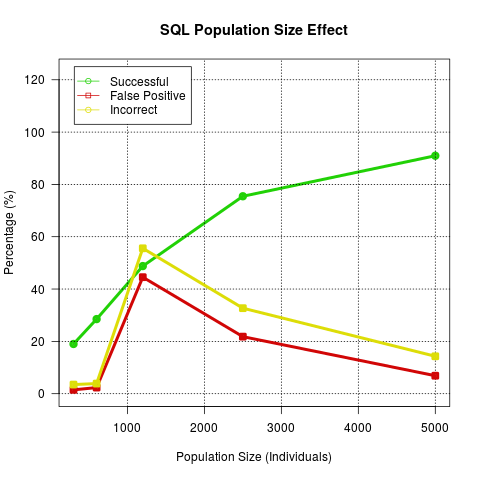
\includegraphics[width=225px]{./assets/results/ga/pop/Results_SQL.png}}
	\subfloat{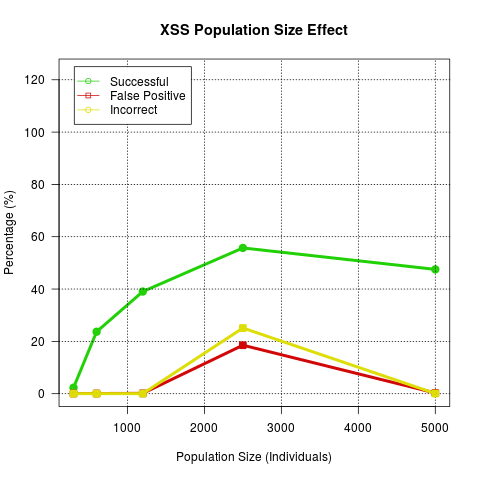
\includegraphics[width=225px]{./assets/appendix/fullresults/ga/pop/Results_XSS.png}}
	\\
	\subfloat{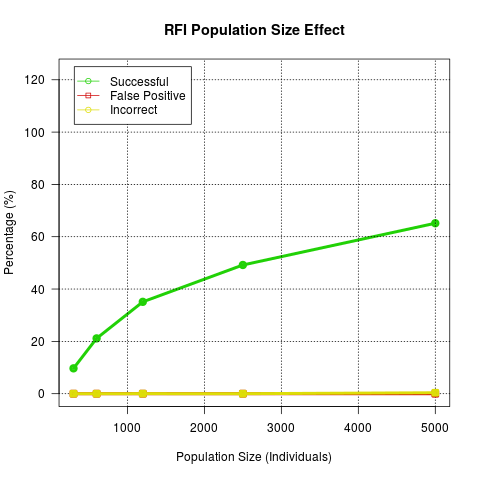
\includegraphics[width=225px]{./assets/appendix/fullresults/ga/pop/Results_RFI.png}}
	\caption{Effects of Population Size on Detection (Appendix \ref{app:sqlPopulationText},\ref{app:xssPopulationText},\ref{app:rfiPopulationText})}
	\label{fig:resPopSize}
\end{figure}

\newpage
\subsubsection{Generations} \label{sec:resGeneration}

The amount of generations also significantly matters because it is the amount of times the genetic algorithm will run.  The more generations, the more likely the algorithm can produce better results and improve upon the existing results (Figure \ref{fig:resGenerations}).

\begin{figure}[hb]
	\centering
	\subfloat{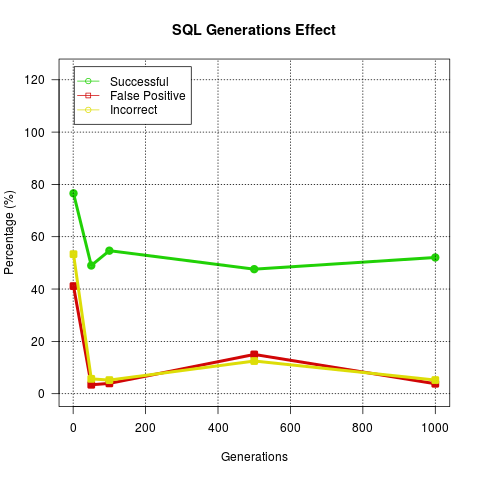
\includegraphics[width=225px]{./assets/results/ga/generations/Results_SQL.png}}
	\subfloat{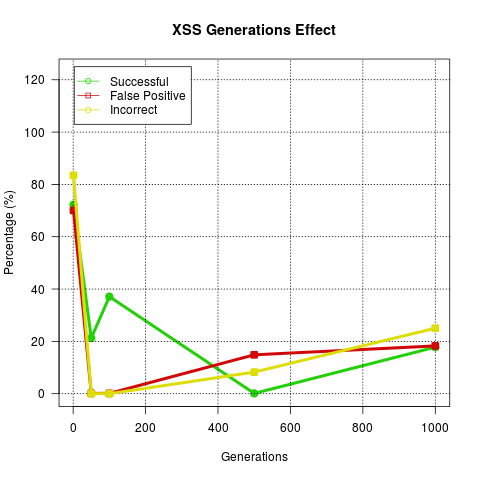
\includegraphics[width=225px]{./assets/appendix/fullresults/ga/generations/Results_XSS.png}}
	\\
	\subfloat{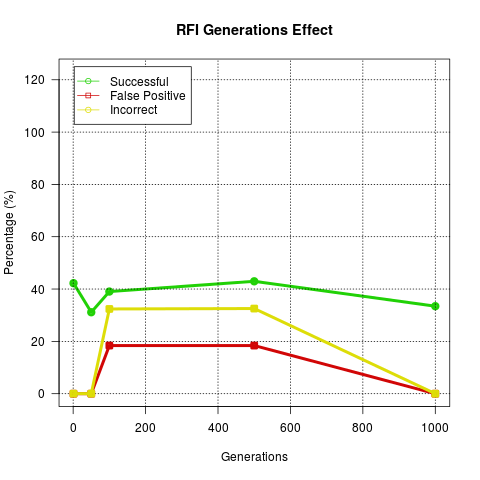
\includegraphics[width=225px]{./assets/appendix/fullresults/ga/generations/Results_RFI.png}}
	\caption{Effects of Generations on Detection (Appendix \ref{app:sqlGenerationText},\ref{app:xssGenerationText},\ref{app:rfiGenerationText})}
	\label{fig:resGenerations}
\end{figure}

\newpage
\subsubsection{Mutation Rate} \label{sec:resMutation}

If the mutation rate is too high then the genetic algorithm basically becomes a random search, while having no mutation rate at all will result in a lack of genetic diversity, with the production of new bitstrings only being a result of crossovers.  It is very difficult to determine a single mutation rate to get the best results and more often than not this is done by trial and error like the following tests will perform \cite{aNewStrategy}.  Mutation rates are typically set to a very low amount since it is on a per allele basis and you would not want to randomize every single bit in a signature and so a value between 0.0 and 1.0\% is often used with 1.0\% being quite high (Figure \ref{fig:resMutation}) \cite{optimizationOfControlParameters}.

\newpage
\begin{figure}[hb]
	\centering
	\subfloat{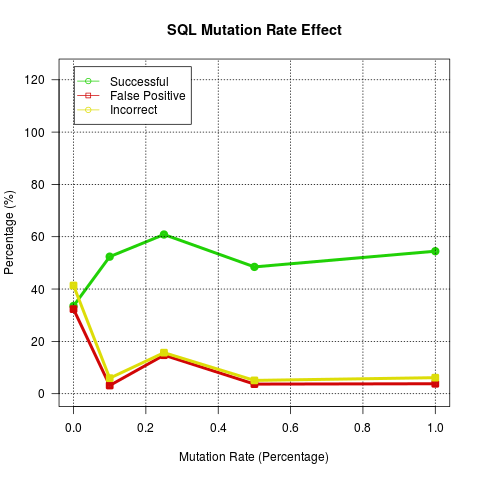
\includegraphics[width=225px]{./assets/results/ga/mutation/Results_SQL.png}}
	\subfloat{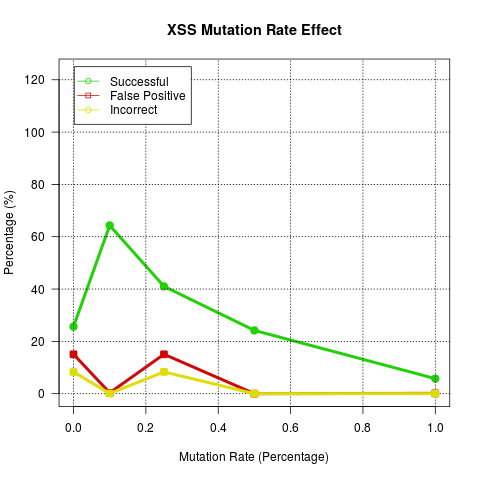
\includegraphics[width=225px]{./assets/appendix/fullresults/ga/mutation/Results_XSS.png}}
	\\
	\subfloat{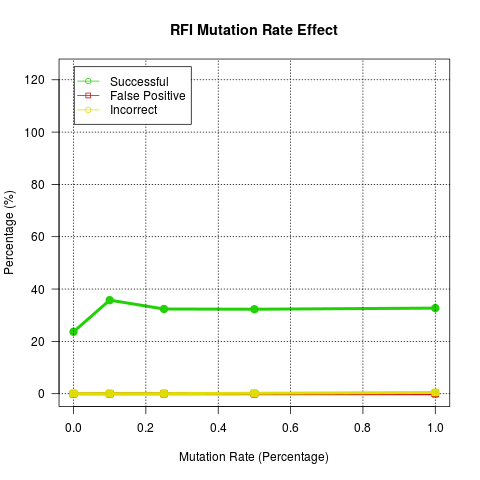
\includegraphics[width=225px]{./assets/appendix/fullresults/ga/mutation/Results_RFI.png}}
	\caption{Effects of Mutation Rate on Detection (Appendix \ref{app:sqlMutationText},\ref{app:xssMutationText},\ref{app:rfiMutationText})}
	\label{fig:resMutation}
\end{figure}

\newpage
\subsubsection{Elitist Pool} \label{sec:resElitist}

The more of the better performing population that survives to the next generation the more likely the change of selecting strong individuals to produce new individuals of a similar or greater strength.  However, if the preservation amount of the population is too much than it may not be able to improve very quickly and the overall search may stagnate.  Sometimes this is also referred to as a generation gap (Figure \ref{fig:resElitist}) \cite{optimizationOfControlParameters}.

\begin{figure}[hb]
	\centering
	\subfloat{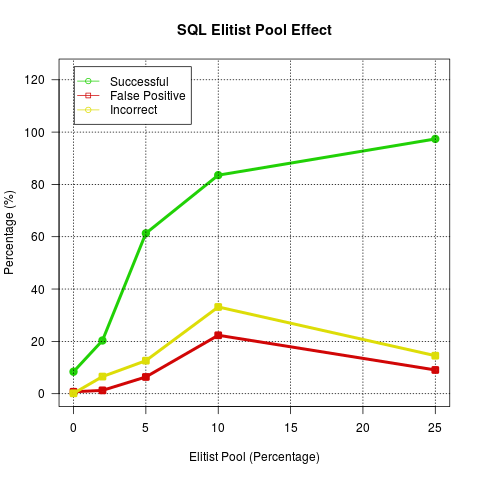
\includegraphics[width=215px]{./assets/results/ga/elitist/Results_SQL.png}}
	\subfloat{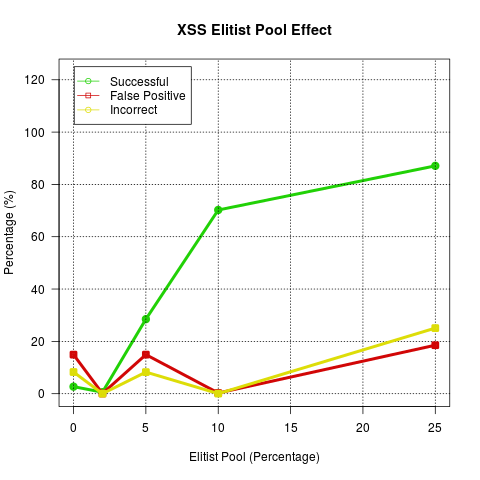
\includegraphics[width=215px]{./assets/appendix/fullresults/ga/elitist/Results_XSS.png}}
	\\
	\subfloat{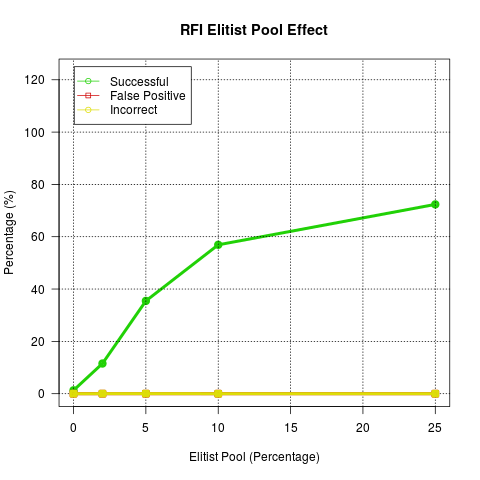
\includegraphics[width=215px]{./assets/appendix/fullresults/ga/elitist/Results_RFI.png}}
	\caption{Effects of Elitist Pool on Detection (Appendix \ref{app:sqlElitistText},\ref{app:xssElitistText},\ref{app:rfiElitistText})}
	\label{fig:resElitist}
\end{figure}

\newpage
\subsection{Combining Multiple Signature Sets} \label{sec:resIteration}

One of the claimed advantages of the genetic algorithm approach, and a big reason why it can work well is because the genetic algorithm can produce new signatures in order to keep appending to an existing set to increase the breadth of detection.  For this reason, running the algorithm multiple times and combining the signatures should result in more detections, but may also result in increased false positives and incorrect detections due to many poor signatures being stored along with one another (Figure \ref{fig:resIterations}).

\begin{figure}[hb]
	\centering
	\subfloat{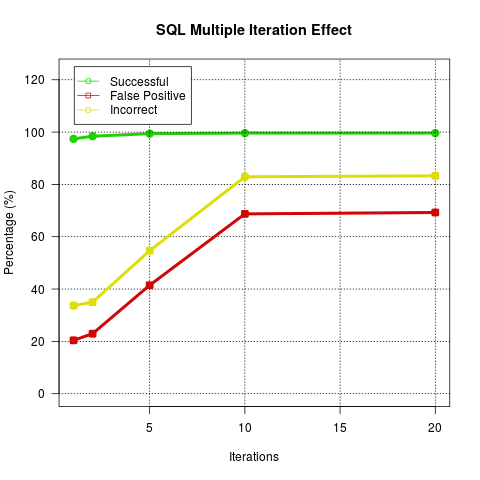
\includegraphics[width=200px]{./assets/results/ga/iterations/Results_SQL.png}}
	\subfloat{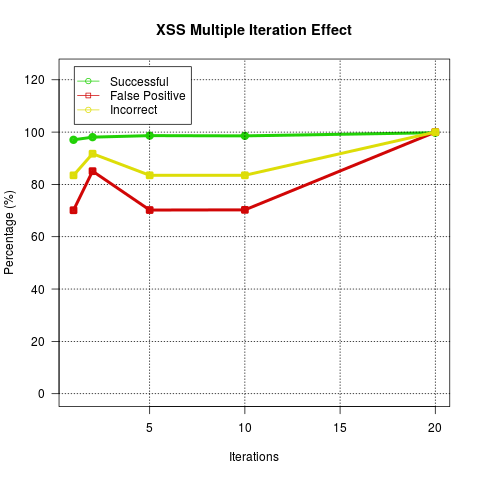
\includegraphics[width=200px]{./assets/appendix/fullresults/ga/iterations/Results_XSS.png}}
	\\
	\subfloat{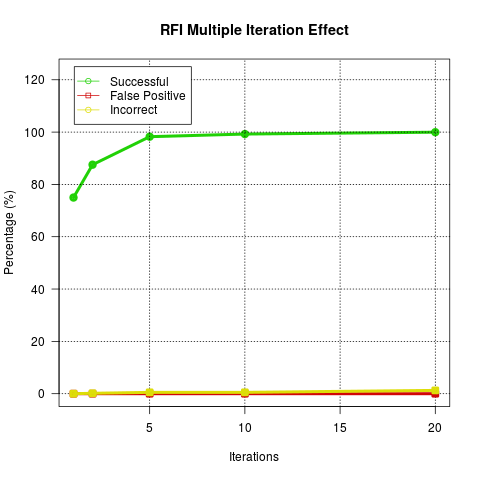
\includegraphics[width=200px]{./assets/appendix/fullresults/ga/iterations/Results_RFI.png}}
	\caption{Effects of Multiple Iterations on Detection (Appendix \ref{app:sqlIterationText},\ref{app:xssIterationText},\ref{app:rfiIterationText})}
	\label{fig:resIterations}
\end{figure}

\newpage
\subsection{Bitstring Segment Length Effects} \label{sec:resSegment}

Because the genetic algorithm is able to detect additional attacks by generating new signatures, if the number of possible signature combinations is less thanks to the segment lengths, then it would be more likely to generate these signatures that match with the training or testing attacks.  However it also opens up the possibility of making it easier to generate poor signatures due to a smaller search space, as well as potentially artificially increase results due to segment overflows (Figure \ref{fig:resLengthSQL},\ref{fig:resLengthXSS},\ref{fig:resLengthRFI}).

\begin{figure}[hb]
	\centering
	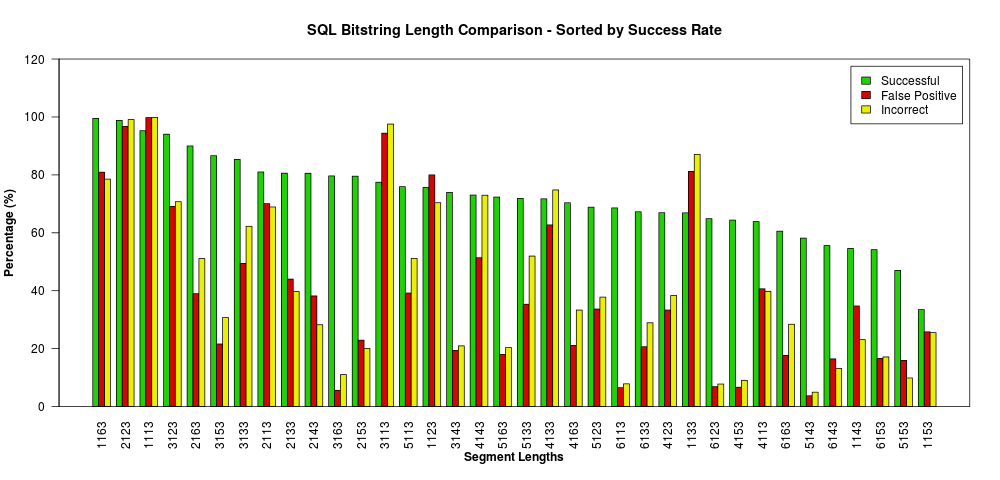
\includegraphics[width=450px]{./assets/results/ga/bitlength/Results_SuccessRate_SQL.png}
	\caption{Effects of Different Segment Lengths on Detecting SQLi (Appendix \ref{app:sqlBitstringTest})}
	\label{fig:resLengthSQL}
\end{figure}

\newpage
\begin{figure}[H]
	\centering
	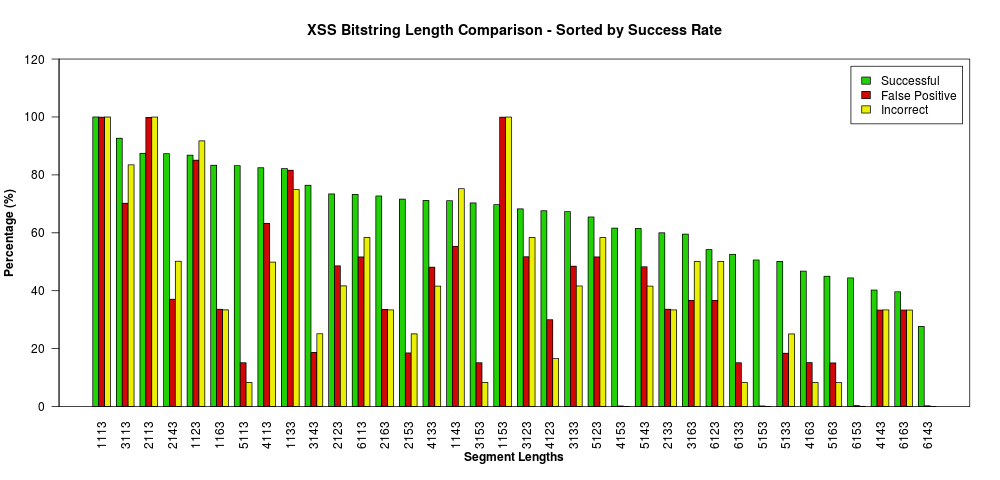
\includegraphics[width=450px]{./assets/appendix/fullresults/ga/bitlength/Results_SuccessRate_XSS.png}
	\caption{Effects of Different Segment Lengths on Detecting XSS (Appendix \ref{app:xssBitstringTest})}
	\label{fig:resLengthXSS}
\end{figure}

\begin{figure}[H]
	\centering
	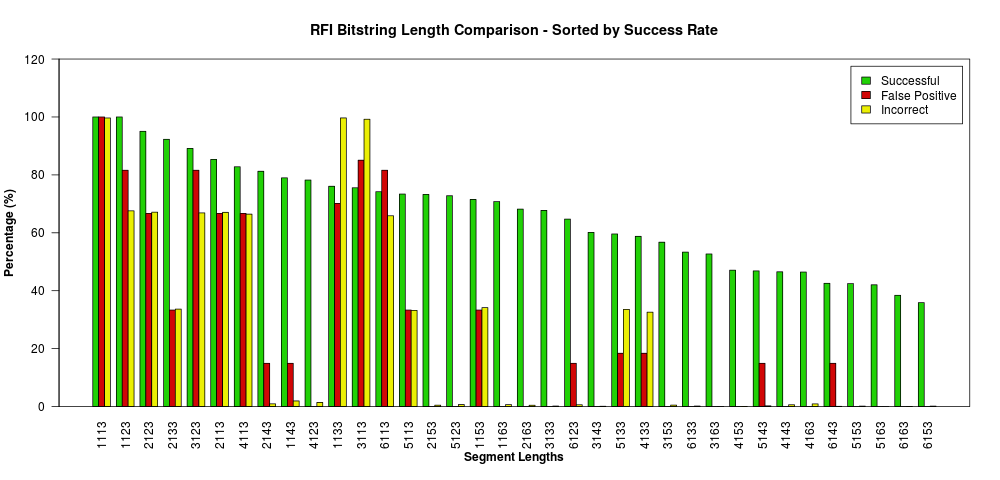
\includegraphics[width=450px]{./assets/appendix/fullresults/ga/bitlength/Results_SuccessRate_RFI.png}
	\caption{Effects of Different Segment Lengths on Detecting RFI (Appendix \ref{app:rfiBitstringTest})}
	\label{fig:resLengthRFI}
\end{figure}

\newpage
\section{Random Permutations with Fitness} \label{sec:resRand}

The genetic algorithm approach works because of the ability to randomly generate new signatures using fitness to weed out the bad signatures, so it would be very interesting to compare the approach with just simply generating all possible combinations and only using the bitstrings that performed well using the same fitness algorithm used in the genetic algorithm.  This could potentially avoid the complexity and computation time that comes along with a genetic algorithm (Algorithm \ref{alg:fitness}), (Figure \ref{fig:resRand}).

\begin{figure}[hb]
	\centering
	\subfloat{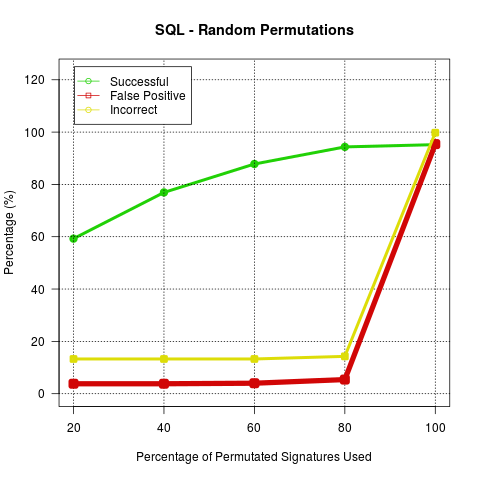
\includegraphics[width=205px]{./assets/results/rand/Results_SQL.png}}
	\subfloat{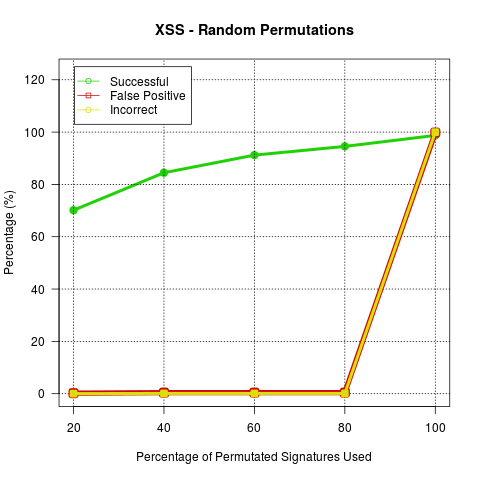
\includegraphics[width=205px]{./assets/appendix/fullresults/rand/Results_XSS.png}}
	\\
	\subfloat{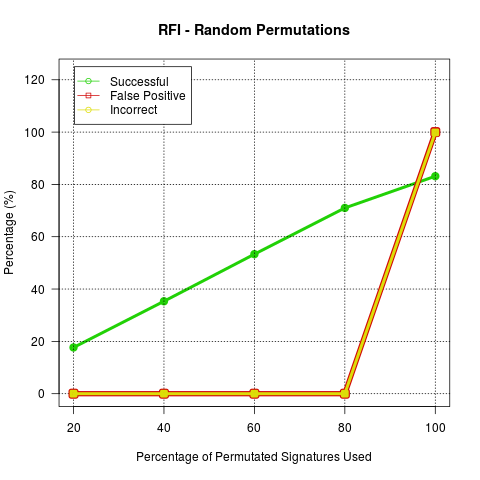
\includegraphics[width=205px]{./assets/appendix/fullresults/rand/Results_RFI.png}}
	\caption{Permutation of Bitstrings for Detection (Appendix \ref{app:sqlRandomText},\ref{app:xssRandomText},\ref{app:rfiRandomText})}
	\label{fig:resRand}
\end{figure}

\section{Support Vector Machine}

For the testing of the support vector machine it was not necessary to average together multiple results as there are no random elements in the algorithm and so the same results are produced every time.  All tests used the same testing data to verify the training process as well as the same training data whenever the required amount of requests did not exceed the amount of used in the genetic algorithms training set.  When doing the genetic algorithm testing it was possible to measure changes by adjusting the algorithm's parameters but in the case of the SVM this is not the case and so instead manipulating the training data will allow for observations on any changes in performance.

\begin{table}
	\begin{tabular}{|p{2.0in}|p{1.125in}|p{1.125in}|p{1.125in}|}
	\hline
	\textbf{Test} & \textbf{\# of requests of intended detection type} & \textbf{\# of requests of incorrect detection type} & \textbf{\# of requests of non-attacks} \\
	\hhline{|=|=|=|=|}
	\textbf{GA Compairson (30\%/30\%/30\%/10\%)} & \textbf{$x$} & \textbf{$2x$} & \textbf{$y$} \\
	\hline
	\textbf{Increasing Non-Threats} & 300 & 600 & \textbf{$x$} \\
	\hline
	\textbf{Increasing Incorrect-Threats} & 300 & \textbf{$2x$} & 350 \\
	\hline
	\end{tabular}
	\caption{Parameters used in each Support Vector Machine Test, the \textbf{$x$} and \textbf{$y$} both signify independent variables, where \textbf{$x$} and \textbf{$y$} are not necessarily the same}
	\label{tab:svmTestParameters}
\end{table}

\begin{figure}[hb]
	\centering
	\subfloat{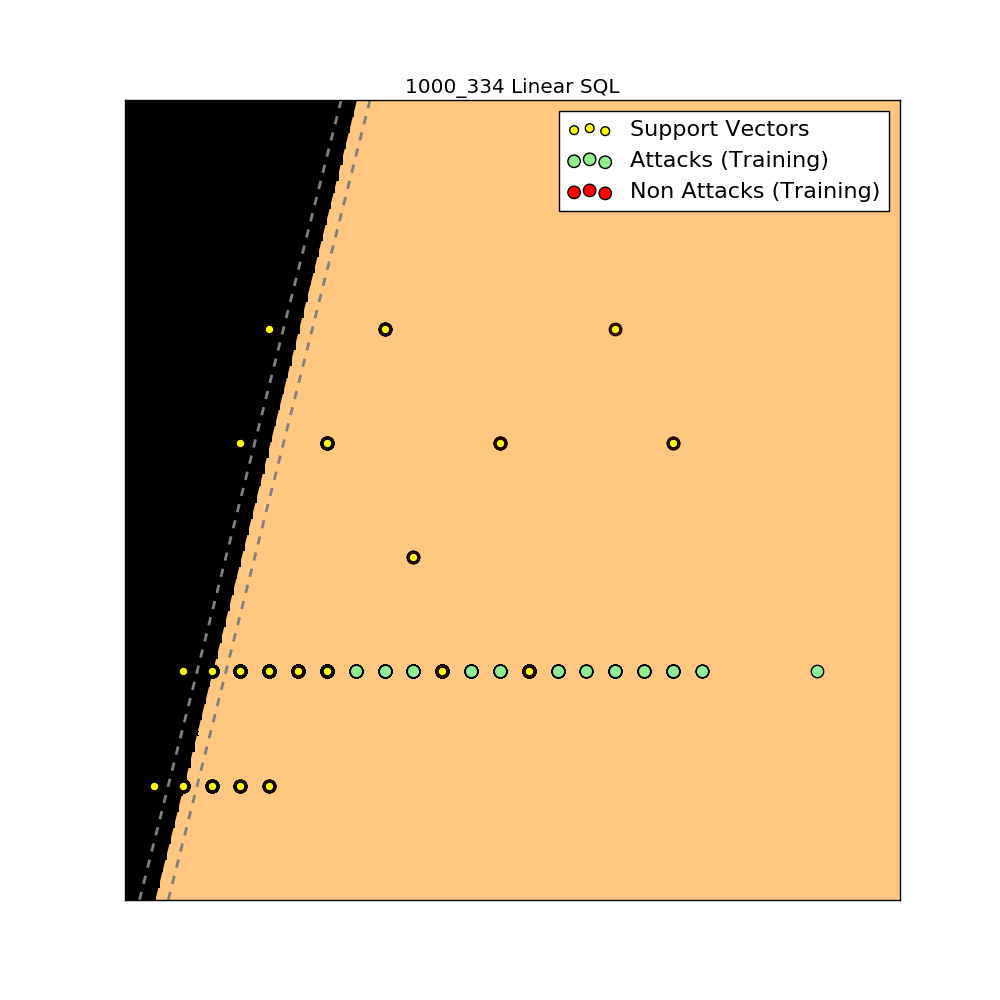
\includegraphics[width=150px]{./assets/results/svm/comparison/linear.png}}
	\subfloat{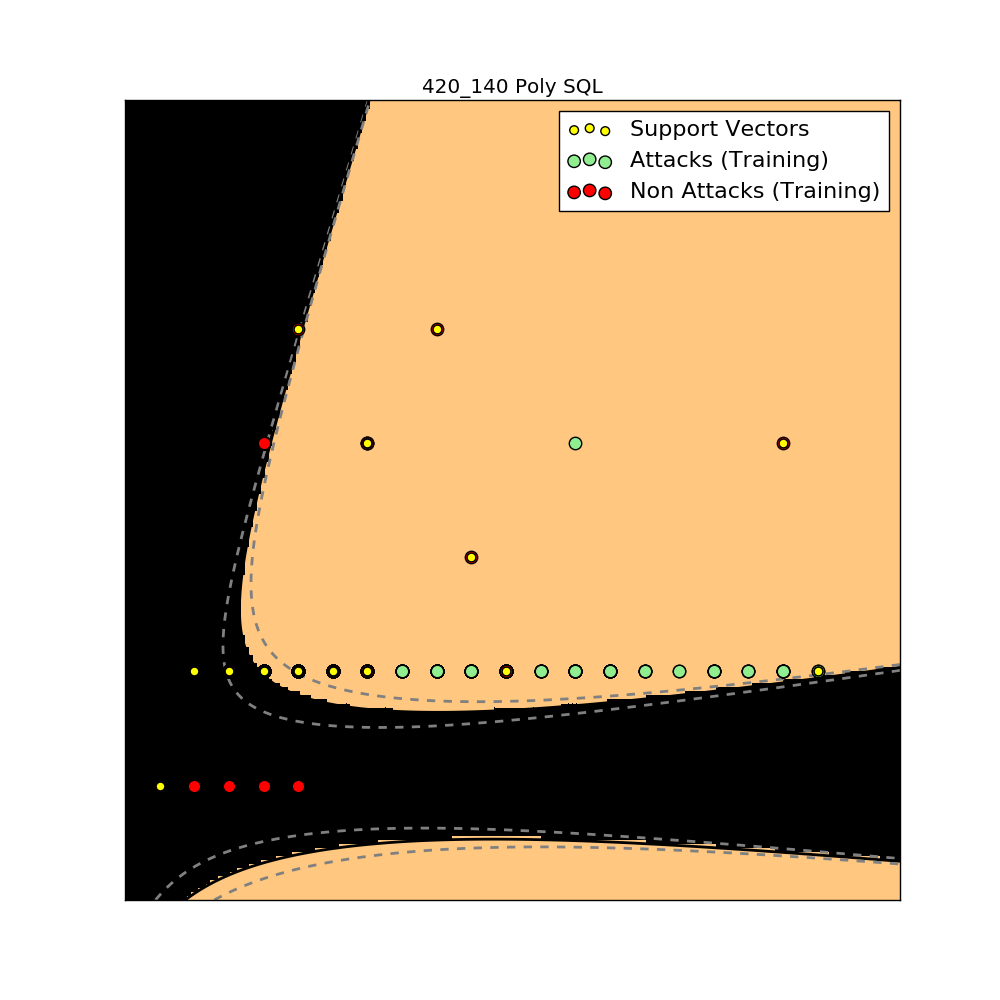
\includegraphics[width=150px]{./assets/results/svm/comparison/poly.png}}
	\subfloat{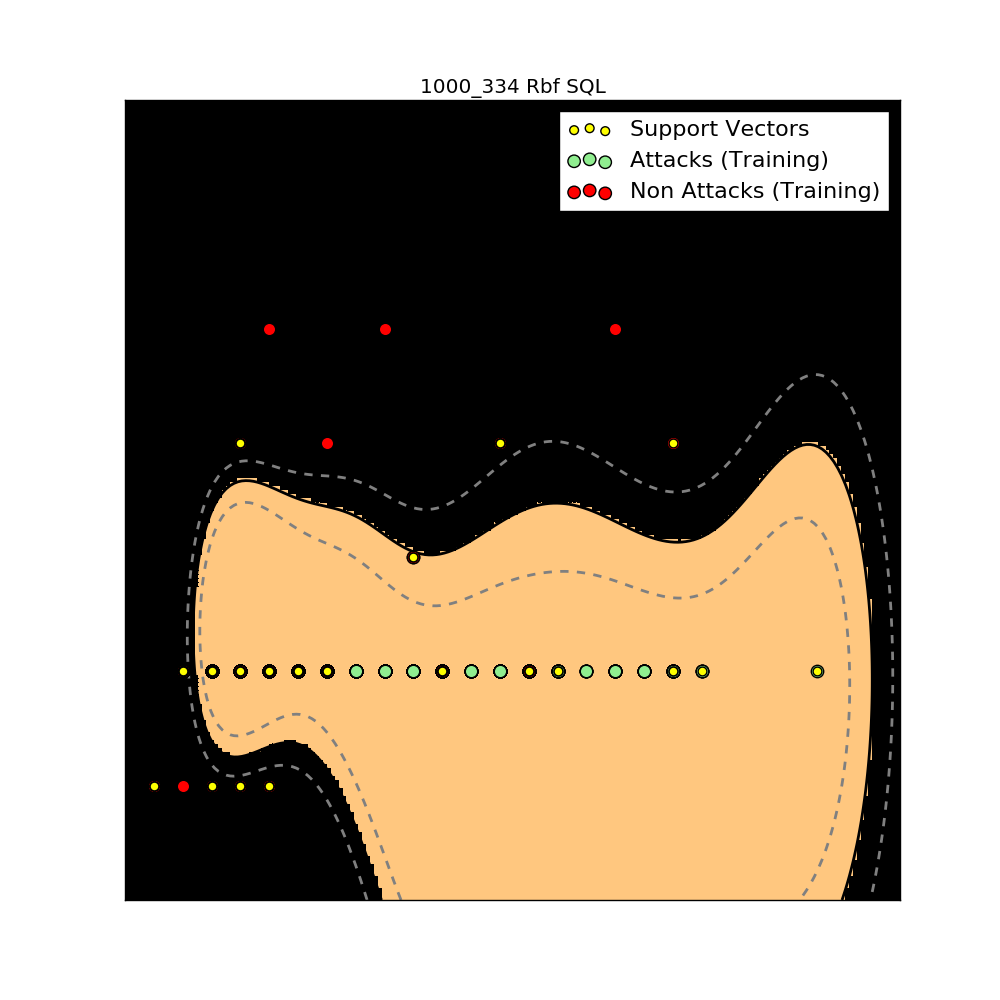
\includegraphics[width=150px]{./assets/results/svm/comparison/rbf.png}}
	\caption{Classifier Output, Linear: 1000\_334, Poly: 420\_140, RBF: 1000\_334}
	\label{fig:resClassifiers}
\end{figure}

\newpage
\subsection{Comparison with Genetic Algorithm} \label{sec:resComparison}

Obtaining the first results uses the same proportions of attack types for training as in the genetic algorithm training set of 30\% for each attack type and 10\% remaining is non-threats. The purpose of this test is to create as fair a comparison as possible with the genetic algorithm (Figure \ref{fig:resComparisonSQL}, \ref{fig:resComparisonXSS},\ref{fig:resComparisonRFI}).  The output classifier for the best performing instance of each kernel is also included (Figure \ref{fig:resClassifiers}).

\begin{figure}[H]
	\centering
	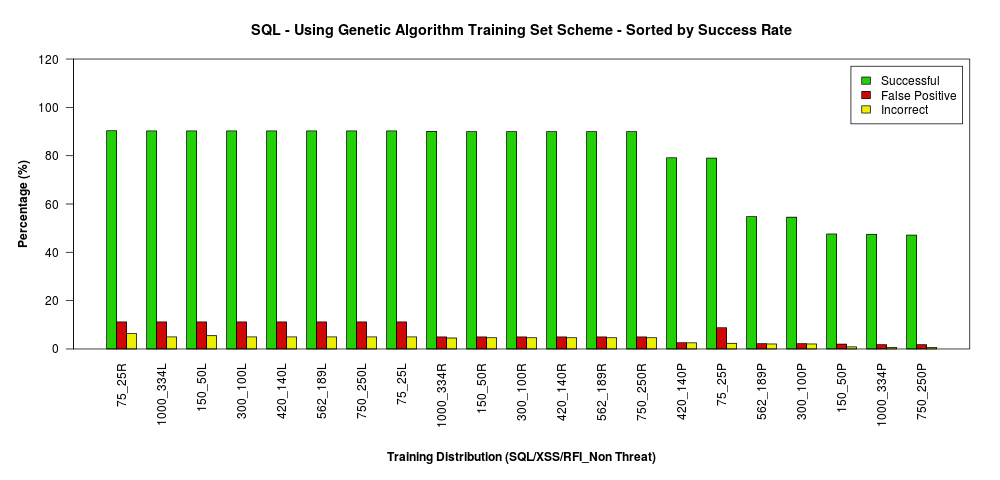
\includegraphics[width=450px]{./assets/results/svm/comparison/Results_SQL.png}
	\caption{Genetic Algorithm and SVM comparison for SQLi Detection (Appendix \ref{app:sqlComparisonText})}
	\label{fig:resComparisonSQL}
\end{figure}

\newpage
\begin{figure}[H]
	\centering
	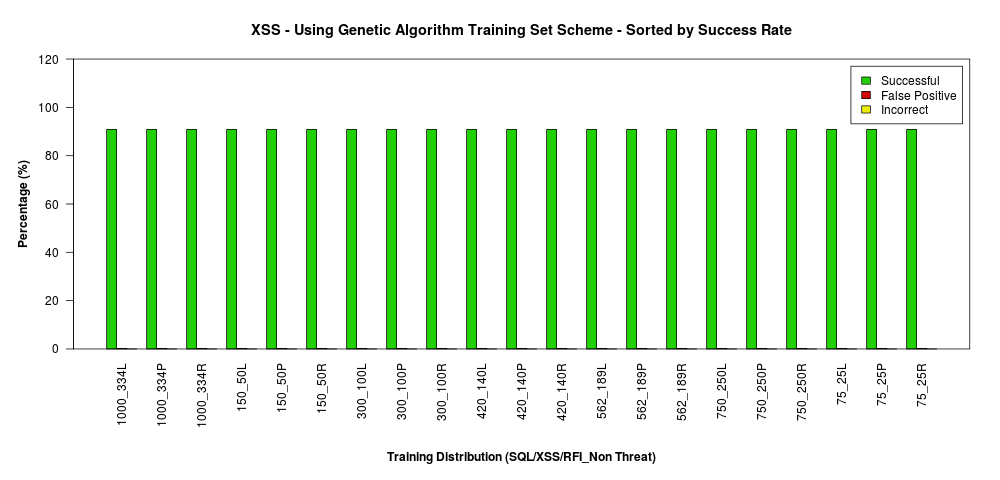
\includegraphics[width=450px]{./assets/appendix/fullresults/svm/comparison/Results_XSS.png}
	\caption{Genetic Algorithm and SVM comparison for XSS Detection (Appendix \ref{app:xssComparisonText})}
	\label{fig:resComparisonXSS}
\end{figure}

\begin{figure}[H]
	\centering
	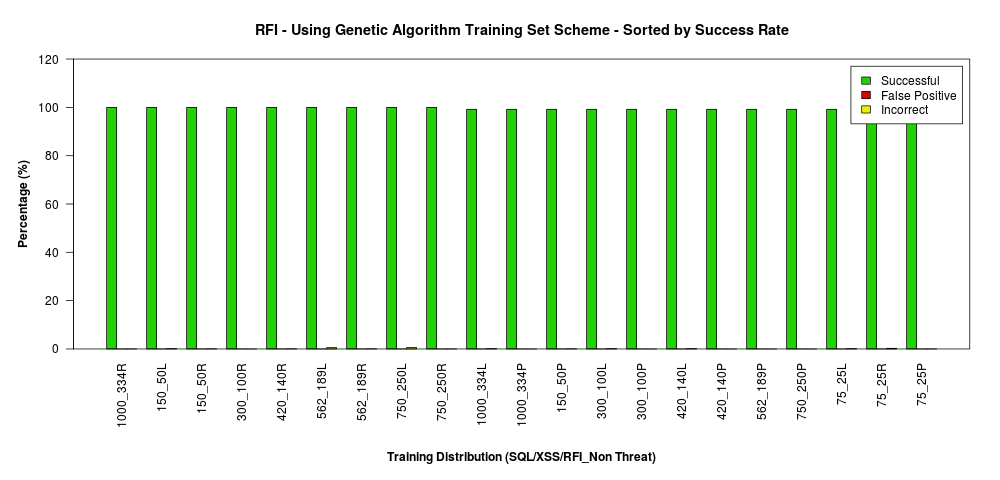
\includegraphics[width=450px]{./assets/appendix/fullresults/svm/comparison/Results_RFI.png}
	\caption{Genetic Algorithm and SVM comparison for RFI Detection (Appendix \ref{app:rfiComparisonText})}
	\label{fig:resComparisonRFI}
\end{figure}

\newpage
\subsection{Increasing Non-Threats} \label{sec:resNonThreat}

Increasing the amount of non-threats in the training data should create a classifier that is more resilient to detecting false positives, the more training data the less likely false positives should occur (Figure \ref{fig:resFalseSQL},\ref{fig:resFalseXSS},\ref{fig:resFalseRFI}).

\begin{figure}[H]
	\centering
	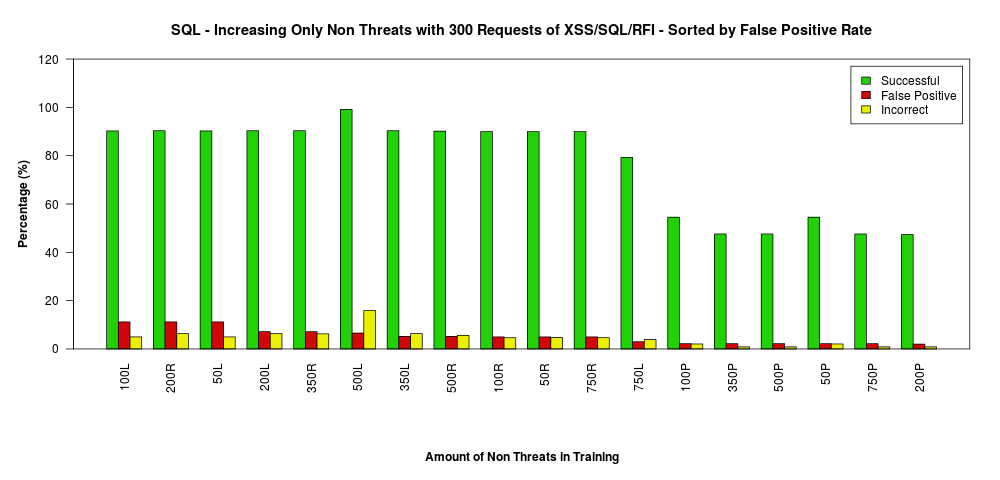
\includegraphics[width=450px]{./assets/results/svm/nonthreat/Results_SQL.png}
	\caption{Effects of increasing non-threat training data in SVM for SQLi detection (Appendix \ref{app:sqlNonThreatText})}
	\label{fig:resFalseSQL}
\end{figure}

\newpage
\begin{figure}[H]
	\centering
	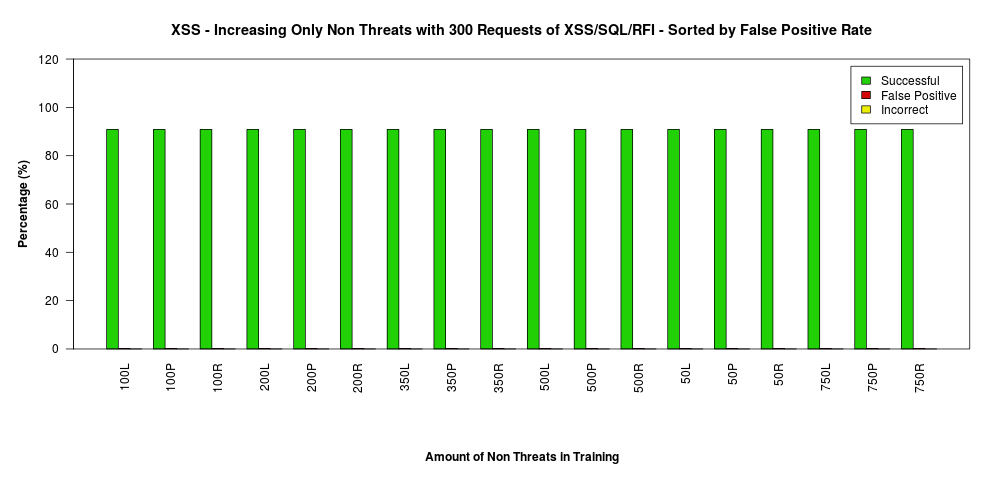
\includegraphics[width=450px]{./assets/appendix/fullresults/svm/nonthreat/Results_XSS.png}
	\caption{Effects of increasing non-threat training data in SVM for XSS detection (Appendix \ref{app:xssNonThreatText})}
	\label{fig:resFalseXSS}
\end{figure}

\begin{figure}[H]
	\centering
	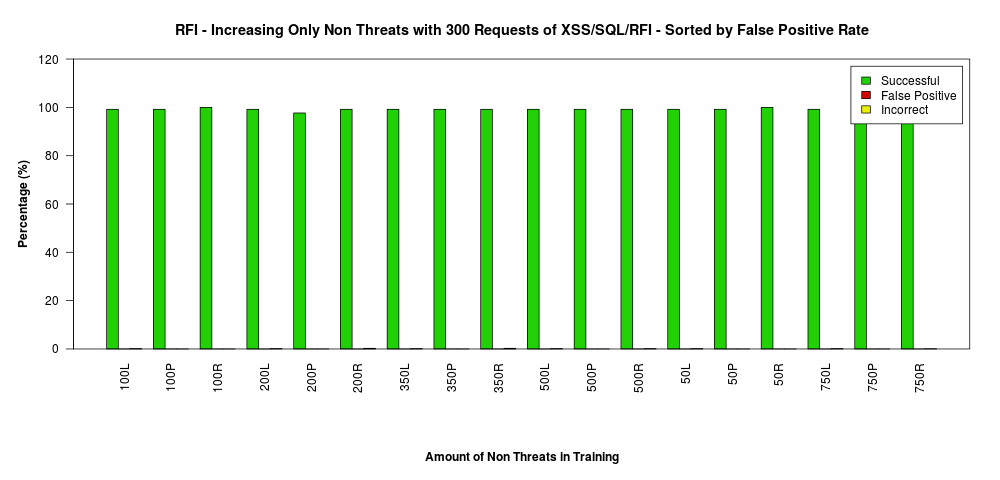
\includegraphics[width=450px]{./assets/appendix/fullresults/svm/nonthreat/Results_RFI.png}
	\caption{Effects of increasing non-threat training data in SVM for RFI detection (Appendix \ref{app:rfiNonThreatText})}
	\label{fig:resFalseRFI}
\end{figure}

\newpage
\subsection{Increasing Incorrect-Threats} \label{sec:resIncorrect}

Similar to the last test, the more threats in the training data that are not the one we are looking for, hopefully the less likely it is for the classifier to incorrectly identify an attack (Figure \ref{fig:resIncorrectSQL},\ref{fig:resIncorrectXSS},\ref{fig:resIncorrectRFI}).

\begin{figure}[H]
	\centering
	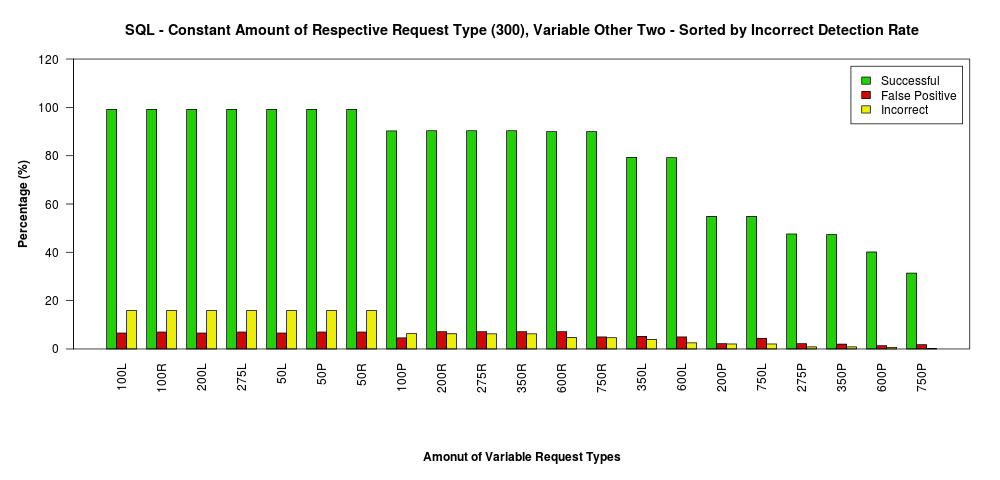
\includegraphics[width=450px]{./assets/results/svm/incorrect/Results_SQL.png}
	\caption{Effects of increasing incorrect attack training data in SVM for SQLi detection (Appendix \ref{app:sqlIncorrectThreatText})}
	\label{fig:resIncorrectSQL}
\end{figure}

\newpage
\begin{figure}[H]
	\centering
	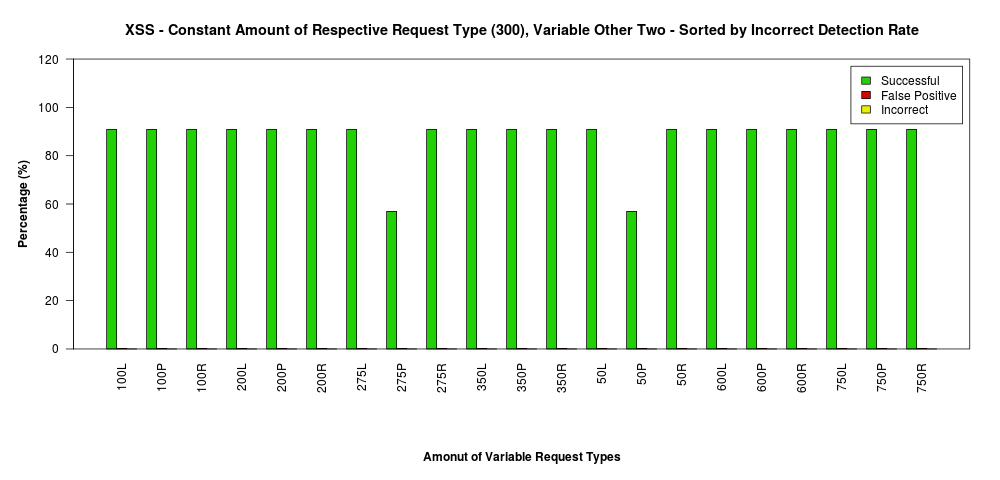
\includegraphics[width=450px]{./assets/appendix/fullresults/svm/incorrect/Results_XSS.png}
	\caption{Effects of increasing incorrect attack training data in SVM for XSS detection (Appendix \ref{app:xssIncorrectThreatText})}
	\label{fig:resIncorrectXSS}
\end{figure}

\begin{figure}[H]
	\centering
	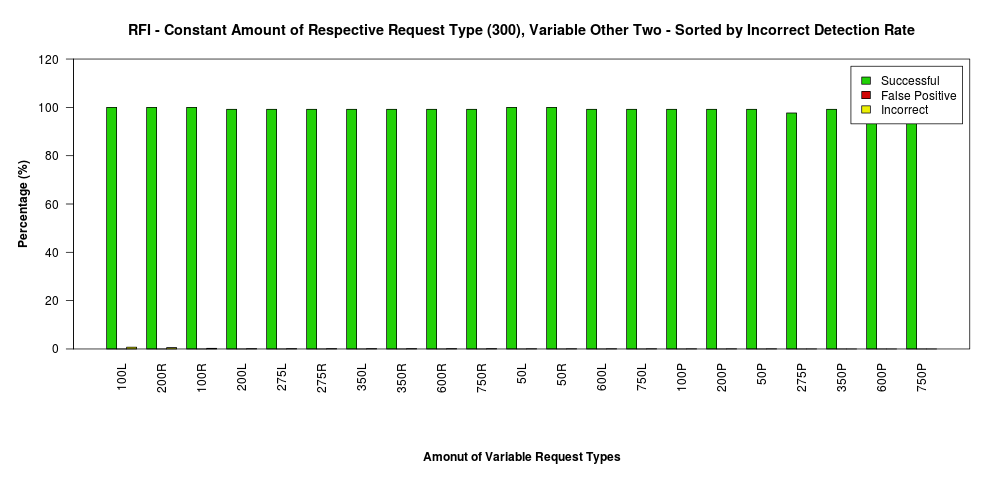
\includegraphics[width=450px]{./assets/appendix/fullresults/svm/incorrect/Results_RFI.png}
	\caption{Effects of increasing incorrect attack training data in SVM for RFI detection (Appendix \ref{app:rfiIncorrectThreatText})}
	\label{fig:resIncorrectRFI}
\end{figure}
 % drafted % results
\chapter{Discussion}

\section{Genetic Algorithm}

\section{Support Vector Machine}
 % drafted % discussion
\chapter{Conclusions}

\section{Conclusions}

\section{Future Work}

 % drafted % conclusion
\begin{appendices}

\chapter{Regular Expression Documentation}
lorem

\chapter{Full Genetic Algorithm Testing Results}


\section{Full Text-Based Results}
lorem
\section{Remaining Graphical Results}
lorem

\chapter{Full Support Vector Machine Testing Results}

\section{Full Text-Based Results}
lorem
\section{Remaining Graphical Results}
lorem







\end{appendices}


% Glossary command does not work in Gummi, will add glossary later if its even needed
%\chapter{Glossary}


%% This adds a line for the Bibliography in the Table of Contents.
\addcontentsline{toc}{chapter}{Bibliography}
%% *** Set the bibliography style. ***
%% (change according to your preference/requirements)
\bibliographystyle{IEEEtran}
%% *** Set the bibliography file. ***
%% ("thesis.bib" by default; change as needed)
\bibliography{thesis}

%% *** NOTE ***
%% If you don't use bibliography files, comment out the previous line
%% and use \begin{thebibliography}...\end{thebibliography}.  (In that
%% case, you should probably put the bibliography in a separate file and
%% `\include' or `\input' it here).

\end{document}
